%%%%%%%%%%%%%%%%%%%%%%%%%%%%%%%%%%%%%%%%%
% Make sure to edit document variables in the Thesis.cls file
%
%%%%%%%%%%%%%%%%%%%%%%%%%%%%%%%%%%%%%%%%%

%----------------------------------------------------------------------------------------
%	PACKAGES AND OTHER DOCUMENT CONFIGURATIONS
%----------------------------------------------------------------------------------------

\documentclass[12pt, oneside]{Thesis} % The default font size and one-sided printing (no margin offsets)

\graphicspath{{Figures/}} % Specifies the direcory where pictures are stored
\usepackage{epstopdf}
\usepackage{titlesec}
\usepackage[square, numbers, comma, sort&compress]{natbib}
\usepackage[ruled,boxed]{algorithm2e}
\usepackage{enumitem,amsmath,amsthm}
\usepackage{amssymb}
 % Use the natbib reference package - read up on this to edit the reference style; if you want text (e.g. Smith et al., 2012) for the in-text references (instead of numbers), remove 'numbers' 
%\hypersetup{linkcolor=black,urlcolor=black,citecolor=black,colorlinks=true} % Colors hyperlinks in blue - change to black if annoying
\title{\ttitle} % Defines the thesis title - don't touch this
%\long\def \/*#1*/{}
%\titlespacing*{\chapter}
\titlespacing*{\chapter}{0pt}{-80pt}{0pt}
\begin{document}
\pagestyle{plain}
\frontmatter % Use roman page numbering style (i, ii, iii, iv...) for the pre-content pages

\setstretch{1.2} % Line spacing of 1.3

% Define the page headers using the FancyHdr package and set up for one-sided printing
%\fancyhead{} % Clears all page headers and footers
%\rhead{\thepage} % Sets the right side header to show the page number
%\lhead{} % Clears the left side page header

%\pagestyle{fancy} % Finally, use the "fancy" page style to implement the FancyHdr headers

\newcommand{\HRule}{\rule{\linewidth}{0.5mm}} % New command to make the lines in the title page
%\newtheorem{lemma}{Lemma}
% \newtheorem{thm}{Theorem}
\newtheorem{thm}{{\break \noindent {\bf Theorem}}}

\newcommand{\loc}   	{ {\mathrm {Loc}} }
\newcommand{\ACONN}   { {\mathrm {A\mbox{-}CONN}} }
\newcommand{\SCONN}   { {\mathrm {S\mbox{-}CONN}} }
\newcommand{\ARCONN}   { {\mathrm {AR\mbox{-}CONN}} }
\newcommand{\SRCONN}   { {\mathrm {SR\mbox{-}CONN}} }
\newcommand{\GV}   { {\mathrm {G=(V,E_G,Loc,p)} }}

\newcommand{\fConn}   	{ {\mathrm {Conn}} }

\newcommand{\nReq}    { {n_{req}} }
\newcommand{\boldS}   { \mathbf{S}}
\newcommand{\DCH}     { {DCH} }

%% -- older paper --

\newcommand{\starEqual}   { {\;{\scriptstyle *} \! =} }
\newcommand{\plusEqual}   { {\;{\scriptstyle +} \! =} }
%\newcommand{\plusplus}    { {\scriptstyle \!+\!+} }

%\newcommand{\starEqual}   { {\; {\mathtt *=}} }
%\newcommand{\plusEqual}   { {\; \mathtt{+=}} }

% --------------------
\newcommand{\set}[1]    {{ \{ #1 \} }}
\newcommand{\iin}[1]    {\hspace*{#1in}}

\newcommand{\ol}[1]     {\overline{#1}}

\newcommand{\Prob}[1]   { {\bf \mathrm{Prob}} \left[ #1 \right] }
\newcommand{\aPr}	{ {\mathrm  {Pr}} }

\newcommand {\nwline} {\hfill\break}
% PDF meta-data
%\hypersetup{pdftitle={\ttitle}}
%\hypersetup{pdfsubject=\subjectname}
%\hypersetup{pdfauthor=\authornames}
%\hypersetup{pdfkeywords=\keywordnames}

%----------------------------------------------------------------------------------------
%	TITLE PAGE
%----------------------------------------------------------------------------------------

\begin{titlepage}
\begin{center}

%\textsc{\LARGE University of Alberta}\\[1.5cm] % University name
%\textsc{\Large Master Thesis}\\[0.5cm] % Thesis type

%\HRule \\[0.4cm] % Horizontal line
{\large \bfseries Probabilistic Connectivity of Underwater Sensor Networks}\\[0.4cm] % Thesis title
%\HRule \\[1.5cm] % Horizontal line
\vspace{0.3 cm}
%\begin{minipage}[0.9\textwidth]
%\begin{flushleft} \large
{\em by}\\
\vspace{0.5 cm}
{Md Asadul Islam}\\ % Author name - remove the \href bracket to remove the link
\vspace{2 cm}
%\end{flushleft}
%\end{minipage}
%\begin{minipage}{0.5\textwidth}
%\begin{flushright} \large
%\emph{Supervisor:} \\
%{Professor Ehab S. Elmallah} % Supervisor name - remove the \href bracket to remove the link  
%\end{flushright}
%\end{minipage}\\[3cm]
 
 \textit{A thesis submitted in partial fulfilment of the requirements for the degree of }\\[0.4cm] % University requirement text
%\textit{in the}\\[0.4cm]
%\groupname\\\deptname\\[2cm] % Research group name and department name
 {\em Master of Science}\\
 
 \vspace*{0.4 cm}
 
 
 {\em Department of Computing Science}\\
  \vspace*{0.4 cm}
 {\em University of Alberta}
%{\large \today}\\[4cm] % Date
%\includegraphics{Logo} % University/department logo - uncomment to place it
 
\vfill
\textcopyright Md Asadul Islam, 2014
\end{center}

\end{titlepage}
%\newpage
%\textbf{Exam Committee}\\\\
%\examname
%
%%----------------------------------------------------------------------------------------
%%	DECLARATION PAGE
%%	Your institution may give you a different text to place here
%%----------------------------------------------------------------------------------------
%%%\comment
%%\Declaration{
%%
%%\addtocontents{toc}{\vspace{1em}} % Add a gap in the Contents, for aesthetics
%%
%%I, \authornames, declare that this thesis titled, '\ttitle' and the work presented in it are my own. I confirm that:
%%
%%\begin{itemize} 
%%\item[\tiny{$\blacksquare$}] This work was done wholly or mainly while in candidature for a research degree at this University.
%%\item[\tiny{$\blacksquare$}] Where any part of this thesis has previously been submitted for a degree or any other qualification at this University or any other institution, this has been clearly stated.
%%\item[\tiny{$\blacksquare$}] Where I have consulted the published work of others, this is always clearly attributed.
%%\item[\tiny{$\blacksquare$}] Where I have quoted from the work of others, the source is always given. With the exception of such quotations, this thesis is entirely my own work.
%%\item[\tiny{$\blacksquare$}] I have acknowledged all main sources of help.
%%\item[\tiny{$\blacksquare$}] Where the thesis is based on work done by myself jointly with others, I have made clear exactly what was done by others and what I have contributed myself.\\
%%\end{itemize}
%% 
%%Signed:\\
%%\rule[1em]{25em}{0.5pt} % This prints a line for the signature
%% 
%%Date:\\
%%\rule[1em]{25em}{0.5pt} % This prints a line to write the date
%%}
%%\endcomment
%\clearpage % Start a new page
%
%%----------------------------------------------------------------------------------------
%%	QUOTATION PAGE
%%----------------------------------------------------------------------------------------

%\pagestyle{empty} % No headers or footers for the following pages
%\end{comment}
%----------------------------------------------------------------------------------------
%	ABSTRACT PAGE
%----------------------------------------------------------------------------------------
\setcounter{page}{2}
\setstretch{2} 
{\Huge \textbf{Abstract}} % Add the "Abstract" page entry to the Contents

%\abstract{\addtocontents{toc}{\vspace{1em}} % Add a gap in the Contents, for aesthetics

Underwater sensor networks (UWSNs) have recently attracted increasing research attention for their potential use in supporting many important applications and services.
Examples include scientific applications such as studies of marine life, industrial applications such as monitoring underwater oil pipelines, humanitarian applications such as search and survey missions, and homeland security applications such as monitoring of ships and port facilities. 
The design of UWSNs, however, faces many challenges due to harsh water environments.
In particular, nodes in such networks are subject to small scale and large scale uncontrollable movements due to water currents.
Since maintaining network connectivity is crucial for performing many tasks that require node collaboration, it becomes important to quantify the likelihood that a network maintains connectivity during some interval of time of interest.
In this thesis, we approach the above challenging problem by adopting a probabilistic model to describe node location uncertainty in semi-mobile and mobile deployments. Using this model, we devise a notion of probabilistic graphs to tackle the problem.
We then formalize four probabilistic network connectivity problems that deal with fully and partially connected networks that may utilize relay nodes.
Using the theory of partial k-trees, we devise algorithms that run in polynomial time, for any fixed k, to solve the formalized problems.
We present simulation experiments to illustrate the use of the devised algorithms in the topological design of UWSNs.

\clearpage
%%----------------------------------------------------------------------------------------
%%	ACKNOWLEDGEMENTS
%%----------------------------------------------------------------------------------------

\setstretch{1.5} % Reset the line-spacing to 1.3 for body text (if it has changed)

\acknowledgements{\addtocontents{toc}{\vspace{1em}} % Add a gap in the Contents, for aesthetics
First of all, I would like to thank my supervisor, Professor Ehab S. Elmallah, for his guidance throughout my Master degree. I am also very grateful for his valuable insight and our frequent
meetings. He also helped me find the topic for this thesis. Above all, he has been a true mentor for me throughout my graduate student life at the University of Alberta and guided me by providing appropriate support to become a successful graduate student. 

Besides my advisor, I would also like to thank the rest of my thesis committee: Professor Lorna Stewart and Professor Janelle Harms for reviewing my work and providing valuable insights and suggestions.

I would like to express my thanks to numerous teacher and friends at the department who have been there for me throughout the coursework and my thesis. I would like to thank Professor Jia You for being a mentor during my coursework. I would also like to particularly mention Mohammed Elmorsy, Israat Haque, Saiful Shuvo and Solimul Chowdhury for their support.

Last but not the least, I would like to thank my family: my wife Musfika Islam Choity for her patience and being with me throughout my thesis and my parents Md Rafiqul Islam and Hamida Khatun, for giving birth to me at the first place and supporting me spiritually throughout my life.


}
\clearpage % Start a new page

%----------------------------------------------------------------------------------------
%	LIST OF CONTENTS/FIGURES/TABLES PAGES
%----------------------------------------------------------------------------------------

%\pagestyle{fancy} % The page style headers have been "empty" all this time, now use the "fancy" headers as defined before to bring them back

%\lhead{\emph{Contents}} % Set the left side page header to "Contents"
\tableofcontents % Write out the Table of Contents
%
%\lhead{\emph{List of Figures}} % Set the left side page header to "List of Figures"
\listoffigures % Write out the List of Figures
%
%\lhead{\emph{List of Tables}} % Set the left side page header to "List of Tables"
\listoftables % Write out the List of Tables

%----------------------------------------------------------------------------------------
%	ABBREVIATIONS
%----------------------------------------------------------------------------------------
%
%\clearpage % Start a new page
%
%\setstretch{1.5} % Set the line spacing to 1.5, this makes the following tables easier to read
%
%\lhead{\emph{Abbreviations}} % Set the left side page header to "Abbreviations"
%\listofsymbols{ll} % Include a list of Abbreviations (a table of two columns)
%{
%\textbf{LAH} & \textbf{L}ist \textbf{A}bbreviations \textbf{H}ere \\
%%\textbf{Acronym} & \textbf{W}hat (it) \textbf{S}tands \textbf{F}or \\
%}
%
%%----------------------------------------------------------------------------------------
%%	PHYSICAL CONSTANTS/OTHER DEFINITIONS
%%----------------------------------------------------------------------------------------
%
%\clearpage % Start a new page
%
%\lhead{\emph{Physical Constants}} % Set the left side page header to "Physical Constants"
%
%\listofconstants{lrcl} % Include a list of Physical Constants (a four column table)
%{
%Speed of Light & $c$ & $=$ & $2.997\ 924\ 58\times10^{8}\ \mbox{ms}^{-\mbox{s}}$ (exact)\\
%% Constant Name & Symbol & = & Constant Value (with units) \\
%}
%
%%----------------------------------------------------------------------------------------
%%	SYMBOLS
%%----------------------------------------------------------------------------------------
%%
%\clearpage % Start a new page
%
%\lhead{\emph{Symbols}} % Set the left side page header to "Symbols"
%
%\listofnomenclature{ll} % Include a list of Symbols (a three column table)
%{
%UWSN & Underwater Sensor Network\\
%ESRT & Event-to-Sink Reliable Transport\\
%TCP & Transmission Control Protocol\\
%CSMA & Carrier Sense Multiple Access\\
%MAC & Media Access Control\\
%CDMA & Code Division Multiple Access \\
%FDMA & Frequency Division Multiple Access\\
%QAM & Quadrature Amplitude Modulation\\
%PSK &  Phase Shift Keying\\
%FSK & Frequency Shift Keying\\
%& \\
%$PES$ & Perfect Elimination Sequence \\
%$A$-$CONN$ & All Node Connectivity \\
%$AR$-$CONN$ & All Node Connectivity with the presence of Relays\\
%$S$-$CONN$ & A Subset of Nodes Connectivity \\
%$SR$-$CONN$ & A Subset of Nodes Connectivity with the presence of Relays\\
%% Symbol & Name & Unit \\
%
% & \\ % Gap to separate the Roman symbols from the Greek
%
%% Symbol & Name & Unit \\
%}

%%----------------------------------------------------------------------------------------
%%	DEDICATION
%%----------------------------------------------------------------------------------------
%
%\setstretch{1.3} % Return the line spacing back to 1.3
%
%\pagestyle{empty} % Page style needs to be empty for this page
%
%\dedicatory{For/Dedicated to/To my\ldots} % Dedication text
%
%\addtocontents{toc}{\vspace{2em}} % Add a gap in the Contents, for aesthetics
%*/
%%----------------------------------------------------------------------------------------
%%	THESIS CONTENT - CHAPTERS
%%----------------------------------------------------------------------------------------
%
\pagestyle{plain}
\setstretch{1.5} 
\mainmatter % Begin numeric (1,2,3...) page numbering
%
%\pagestyle{fancy} % Return the page headers back to the "fancy" style
%
%% Include the chapters of the thesis as separate files from the Chapters folder
%% Uncomment the lines as you write the chapters
%
%\lhead{\emph{Chapter1}}
\chapter{Introduction}
\titlespacing*{\chapter}{0pt}{-50pt}{40pt}
\label{Chapter1} % For referencing the chapter elsewhere, use \ref{Chapter1} 

\lhead{Chapter 1. \emph{Chapter Title Here}} % This is for the header on each page - perhaps a shortened title

%----------------------------------------------------------------------------------------
\begin{quotation}
Underwater Sensor Networks (UWSNs) provide an enabling technology for the development of ocean observation systems. Application domains of UWSNs include military surveillance, disaster prevention, assisted navigation, offshore exploration, tsunami monitoring, oceanographic data collection, to mention a few. Many of the above mentioned applications utilize UWSNs nodes that may move freely with water currents. Thus, node locations at any instant can only be specified probabilistically. When connectivity among some of the sensor nodes is required to perform a given function, the problem of estimating the likelihood that the network achieves such connectivity arises.

In this chapter, we give an overview of UWSNs, highlight some research work done in the area, and discuss some related node mobility  models used by networking researchers in the area. Next, we introduce a probabilistic mobility model that is used to formalize the problems considered in the thesis. We conclude by outlining thesis contributions.
 \end{quotation}
\section{Introduction}
\label{ch1:intro}
In recent years, underwater sensor networks (UWSNs) have attracted considerable attention in networking research.
A typical UWSN is conceived to have a number of sensor nodes that can perform sensing tasks, data storage and processing tasks, and data communication tasks.
Drifters and RAFOS floats (see, e.g., \cite{bower1989evidence}) are examples of devices with no self-controlled mobility that have been used in real oceanography experiments. In addition to such devices, modern UWSNs utilize Autonomous Underwater Vehicles (AUVs) with self-controlled mobility.
Several surveys on the history, architecture, potential applications, and design and implementation challenges of UWSNs appear in \cite{akyildiz2005underwater, partan2007survey, heidemann2012underwater, climent2014underwater, gkikopouli2012survey}.
In this introduction, we highlight some of these aspects to motivate the particular research direction taken in the thesis.



To start, we mention that interest in UWSNs research has been fuelled by many important underwater sensing applications and services that can be supported by such networks.
In  \cite{akyildiz2005underwater} and \cite{heidemann2012underwater}, for example, the domains of applications are classified as follows.
\begin{itemize}
\item \textbf{Scientific applications}: e.g., observing  geological processes on the ocean floor, determining water characteristics (e.g., temperature, salinity, oxygen levels, bacterial and other pollutant content, and dissolved matter), counting or imaging animal life (e.g., micro-organisms, fish or mammals, and coral reef)
\item \textbf{Industrial applications}: e.g., monitoring and control of commercial activities, determining routes for underwater cables, monitoring underwater equipment  and pipelines for oil and mineral extraction, and monitoring commercial fisheries
\item \textbf{Military and homeland security applications}: e.g., monitoring and securing port facilities

\item \textbf{Humanitarian applications}: e.g., search and survey missions, disaster prevention tasks (e.g., tsunami warning to coastal area), identification of seabed hazards, locating dangerous rocks or shoals, and identifying possible mooring locations
\end{itemize}

UWSNs are expected to provide better services in each of the above domains over the traditional approach of deploying underwater sensor devices that record data during a monitoring mission, and then recovering the devices at the end of a mission.
In \cite{akyildiz2005underwater}, the authors point out that compared to this traditional approach, UWSNs provide the following advantages:
\begin{itemize}[noitemsep]
\item supporting real time monitoring, since the observed data can be transmitted shortly after collection,
\item supporting better interaction between onshore control systems and the monitoring devices, and
\item supporting better handling of device failures and misconfigurations.
\end{itemize}
It has also been emphasized in the above survey papers that UWSNs are expected to be sparser than terrestrial wireless sensor networks (WSNs) since individual nodes in UWSNs have significantly more cost compared to nodes in terrestrial WSNs. In addition, many UWSNs are required to cover relatively larger water areas.

The design and implementation of cost effective UWSNs to serve the above applications, however, face a number of challenges.
Some of these challenges are attributed to the current technological limitations of dealing with the underwater communication channel. Other challenges are attributed to the harsh environment of underwater environments.

\textbf{Challenges of the underwater communication channel.} Unlike terrestrial-based WSNs that enjoy low delay and high bandwidth networking devices, UWSNs face significant challenges in getting adequate communication bandwidth.  To see this, we summarize below some of the findings emphasized in \cite{partan2007survey} and  \cite{akyildiz2005underwater} on the use of radio frequency communication, optical communication, and acoustic communication for UWSNs. (All frequencies, bandwidths, distances, and data rates given below are approximate values or ranges to illustrate the main findings.)



\begin{itemize}
\item \textbf{Radio frequency communication.} The majority of radio frequencies suffer strong attenuation in salt water. Long-wave radio (1-100 KHz) can be used for short distances (6-20 m) and low data rates (1 Kbps). Communication with long-wave radio, however, requires large antennas and high transmission power.
In the past, communication to a satellite has been used to send the collected data when an UWSN node floats on water surface after completing a mission.

\item \textbf{Optical communication.} Light is also strongly scattered and absorbed underwater. In \cite{partan2007survey}, it is pointed out that blue-green wavelengths may be used for short-range, high bandwidth connections in extremely clear water.
Thus, optical communication in UWSNs are limited to short distances ($\leq 40$ m) using directed transmission over unobstructed line-of-sight communication.
Low cost optical communication for very short connections (1-2 m) at rates of 57 Kbps has been considered in \cite{fair2006optical, freitag2001acoustic}.

\item \textbf{Acoustic communication.} Sound also suffers from various factors of attenuation, spreading, as well as man-made noise, and ambient noise in underwater. 
Acoustic communication, however, is currently perceived as the most practical method.
In \cite{akyildiz2005underwater}, the authors take a closer look at the capabilities of current acoustic modems. 
They classify the available bandwidth for different distance ranges in UW acoustic channel as follows (for brevity, we use the notation [\textbf{distance range, bandwidth}] to present the classification):  very long [1000 Km, $<$ 1 KHz], long [10-100 Km, 2-5 KHz], medium [1-10 Km, $\approx$ 10 KHz], short [0.1-1 Km, 20-50 KHz], and very short [$<$ 0.1 Km, $>$ 100 KHz].
The speed of sound underwater is approximately 1500 m$/$s, which is $2\times 10^5$ times lower than the speed of light. 
So, acoustic communication suffers from long delays as well.
Standard acoustic transducers can be relatively big in size, heavy weight, and power hungry. In \cite{partan2007survey}, the authors point out that on compact stationary sensor nodes, and space-constraint AUVs, transducers generally cannot be spatially separated far enough to provide full-duplex connections since the transmitted signals will saturate the receiver even when the communication bands are fairly widely separated.
Thus, underwater networks are expected to utilize half-duplex connections.
\end{itemize}

The above challenges in supporting low delay and high data rate communication have triggered research work in almost all areas of the UW networking protocol stack.
The following surveys are particular to UWSNs: Medium Access Control (MAC) protocols \cite{Farrell2012, yunus2010survey, petrioli2008comparative, yigitel2011qos, chen2014}, routing  \cite{ayaz2011survey, pompili2006routing, bayrakdar2011comparative, giantsis2011comparison}, localization \cite{chandrasekhar2006localization, zhou2010efficient, zhou2011scalable, tan2011survey, erol2011performance}, connectivity and coverage \cite{ghosh2008coverage, zhu2012survey}.  Examples of research work done on connectivity, coverage, and deployments appear in \cite{senel2013autonomous, akkaya2009self, ammari2010study, Nazrul2008,  reza2009robust}.


\textbf{Challenges due to node mobility.} To serve the diverse types of applications mentioned above, various types of UWSN deployments are used.
In \cite{heidemann2012underwater}, for example (see, e.g., figure \ref{fig:Exm111}), UWSN deployments are
classified as being either static, semi-mobile, or mobile.
%
Static networks have nodes attached to underwater ground,
anchored buoys, or docks.
%
Semi-mobile networks may have collection of nodes attached to a
free floating buoy. Nodes in semi-mobile networks are subject to small scale
movements.
%
Mobile networks may be composed of drifters with no self mobility
capability, or nodes with mobility capability. Nodes in such networks
are subject to large scale movements.
%
UWSN deployments may occur over many short periods of times (e.g.,
several days at a time), so as to conduct several missions over
a large area of interest.
\begin{figure}[h]
\centering
\includegraphics[width=5 in, height=2.5 in]{UnderwaterScnerio1.pdf}
 \caption{ Example UWSNs.}
 \label{fig:Exm111}
\end{figure}
Maintaining connectivity in such networks is a crucial aspect for performing many tasks that require node collaboration.
Examples of such tasks include localization \cite{teymorian20093d, erol2008multi, isik2009three, zhou2010efficient, zhou2011scalable, erol2011performance}, routing \cite{noh2013vapr, ying2011combining, lee2010pressure, ren2012performance} and coverage \cite{ammari2010study, senel2013autonomous, akkaya2009self, pompili2006deployment}.

In this thesis, we consider semi-mobile and mobile networks.
Our interest is in developing methodologies that allow a designer to analyze the likelihood that a network (or part of it) is connected at a given time interval.
In the next section, we review some work on quantifying node mobility models used by networking researchers for UWSNs.

\section{Node Mobility}
\label{ch1:wounmm}

One may classify node mobility in UWSNs into controllable mobility (C-mobility for short), and uncontrollable mobility (U-mobility).
The simplest type of C-mobility is vertical movements induced by mechanical devices inside a node \cite{erol2008multi, Erol:2007}.
Full 3D C-mobility is enjoyed by AUVs at the expense of node energy consumption.
U-mobility, on the other hand, is primarily due to surface and subsurface water currents, as well as wind.
Findings of real ocean measurements, as well as a large body of analytical results in oceanography have shaped the understanding of networking researchers in this area.


We note that this area is new to networking researchers where the obtained analytical results are rooted in the mathematically deep field of fluid dynamics.
The thesis work makes an effort to summarize some of the important findings in this regard.
Our goal in this section is to foster the idea that numerical values for the probabilistic locality model used throughout the thesis can be deduced from the available empirical measurements of node mobility, and the obtained analytical models that capture the behaviour found in the empirical results.


The probabilistic node locality adopted in the thesis divides the geographic area containing nodes into rectangles of an (imaginary) superimposed grid layout.
After a given time period following network deployment in water, each node $x$ can be in any one of a possible set of grid rectangles, denoted $Loc(x) = \{x[1], x[2],\ldots\}$.
We call $Loc(x)$ the locality set of $x$. 
Thus, depending on the mobility model induced by water currents, node $x$ can be in any possible grid rectangle $x[i]\in Loc(x)$ with a certain probability, denoted $p_x(i)$.


To explain that such probability distribution can be deduced from empirical experiments, we refer to the important work of \cite{bower1989evidence} which has triggered intensive work in the area.
In \cite{bower1989evidence}, the authors report on several observations collected in the Gulf Stream using thirty-seven RAFOS drifters launched off Cape Hatteras.
Mobility of the free floating drifters is tracked for 30 or 45 days.
Among the collected observations, the authors determined the geographic location of each of the 37 drifters at each day of the observation period.
Given the exact geographic location of each drifter in each day, one can superimpose a virtual grid (of some user specified dimensions per rectangle) on the area traversed by the floats and use the reported locations to derive rough values of the probabilities used in our probabilistic locality model.


Next, we present our findings on the use of the available analytical mobility models to derive the probabilities used in our model.
In \cite{bower1989evidence}, the authors observed striking patterns of cross-stream and vertical motion associated with meanders in the Gulf Stream.
Later, in \cite{bower1991simple}, the author introduced a 2D kinematic model that captures many of the important patterns observed in \cite{bower1989evidence} including the effect of meandering sub-surface currents and vortices on free floating drifters.
The introduction of such kinematic model has resulted in a large body of subsequent analytical work in the area.
Recently, this kinematic model has received attention in networking literature.
Following a similar approach, \cite{caruso2008meandering} devised a kinematic mobility model for UWSNs, called the meandering current mobility model.
The model is useful for large coastal environments that span several kilometres.
It captures the strong correlations in mobility of nearby sensor nodes.
In \cite{caruso2008meandering}, the model has been used to analyze several network connectivity, coverage, and localization aspects of UWSNs by simulation.

\textbf{The kinematic model of \cite{caruso2008meandering}}. To explain the model presented in \cite{caruso2008meandering}, we start by recalling some concepts from fluid dynamics (see, e.g., \cite{yunus2013fluid}).
A particle \textit{pathline} is a path followed by an individual particle in a flow.
A \textit{stream} function is a scalar function, denoted  $\psi$, that measures the volume flow rate per unit depth at a point with coordinate $(x,y)$.
Curves where $\psi$ is constant are called \textit{streamlines}.
For steady flows, streamlines and particle paths coincide.
In 2D, a stream function has the property that the $x$ and $y$ velocity vectors ($\dot{x}$ and $\dot{y}$ ) can be obtained by taking partial derivatives of the stream function, as shown below.
The stream function adopted in \cite{caruso2008meandering} utilizes also time (the parameter $t$) to determine the function value, as follows:

\begin{equation}\label{eq:sf}
\psi(x,y,t)=-\tanh{[\frac{y-B(t)\sin(k(x-ct))}{\sqrt{1 + k^2 B^2(t) \cos^2(k(x-ct))}} ]} + cy
\end{equation}
 where $  B(t) = A + \epsilon \cos(\omega t)$  and the $x$ and $y$ velocities are given by
 
 \begin{equation}\label{eq:lf}
\dot{x}=-\frac{\partial \psi}{\partial y} ; \dot{y}=\frac{\partial \psi}{\partial x}
\end{equation}


The trajectory of a node that moves within the current is the solution of the above ordinary differential equations.
We now present the following remarks using the same parameter setting used in \cite{caruso2008meandering}. Namely, $A=1.2, c=0.12, k=\frac{2\pi}{7.5}, \omega=0.4$ and $\epsilon=0.3$, 

\begin{enumerate}
\item For a fixed $t$ (we use $t=0$), a plot of the stream function $\psi$ in $3D$ is shown in figure \ref{fig:kme3d}.
The plot shows that particles deployed at coordinates $x=0$ and $y\in [-2,+2]$ tend to follow sinusoidal pathlines, whereas particles deployed elsewhere may fall into circulations.
\begin{figure}[!htb]
\centering
\includegraphics[width=5 in, height=3 in]{BBC.pdf}
 \caption{ A 3D plot of stream function \ref{eq:sf}}
 \label{fig:kme3d}
\end{figure}

Figure \ref{fig:kme} illustrates the contours of the 3D plots when drawn in 2D.

\item We observe from figure \ref{fig:kme} that any particle deployed in the area shown stays within a strip of vertical height (along the $y$-axis) of $\pm$ 4 Kms.

\begin{figure}[!htb]
\centering
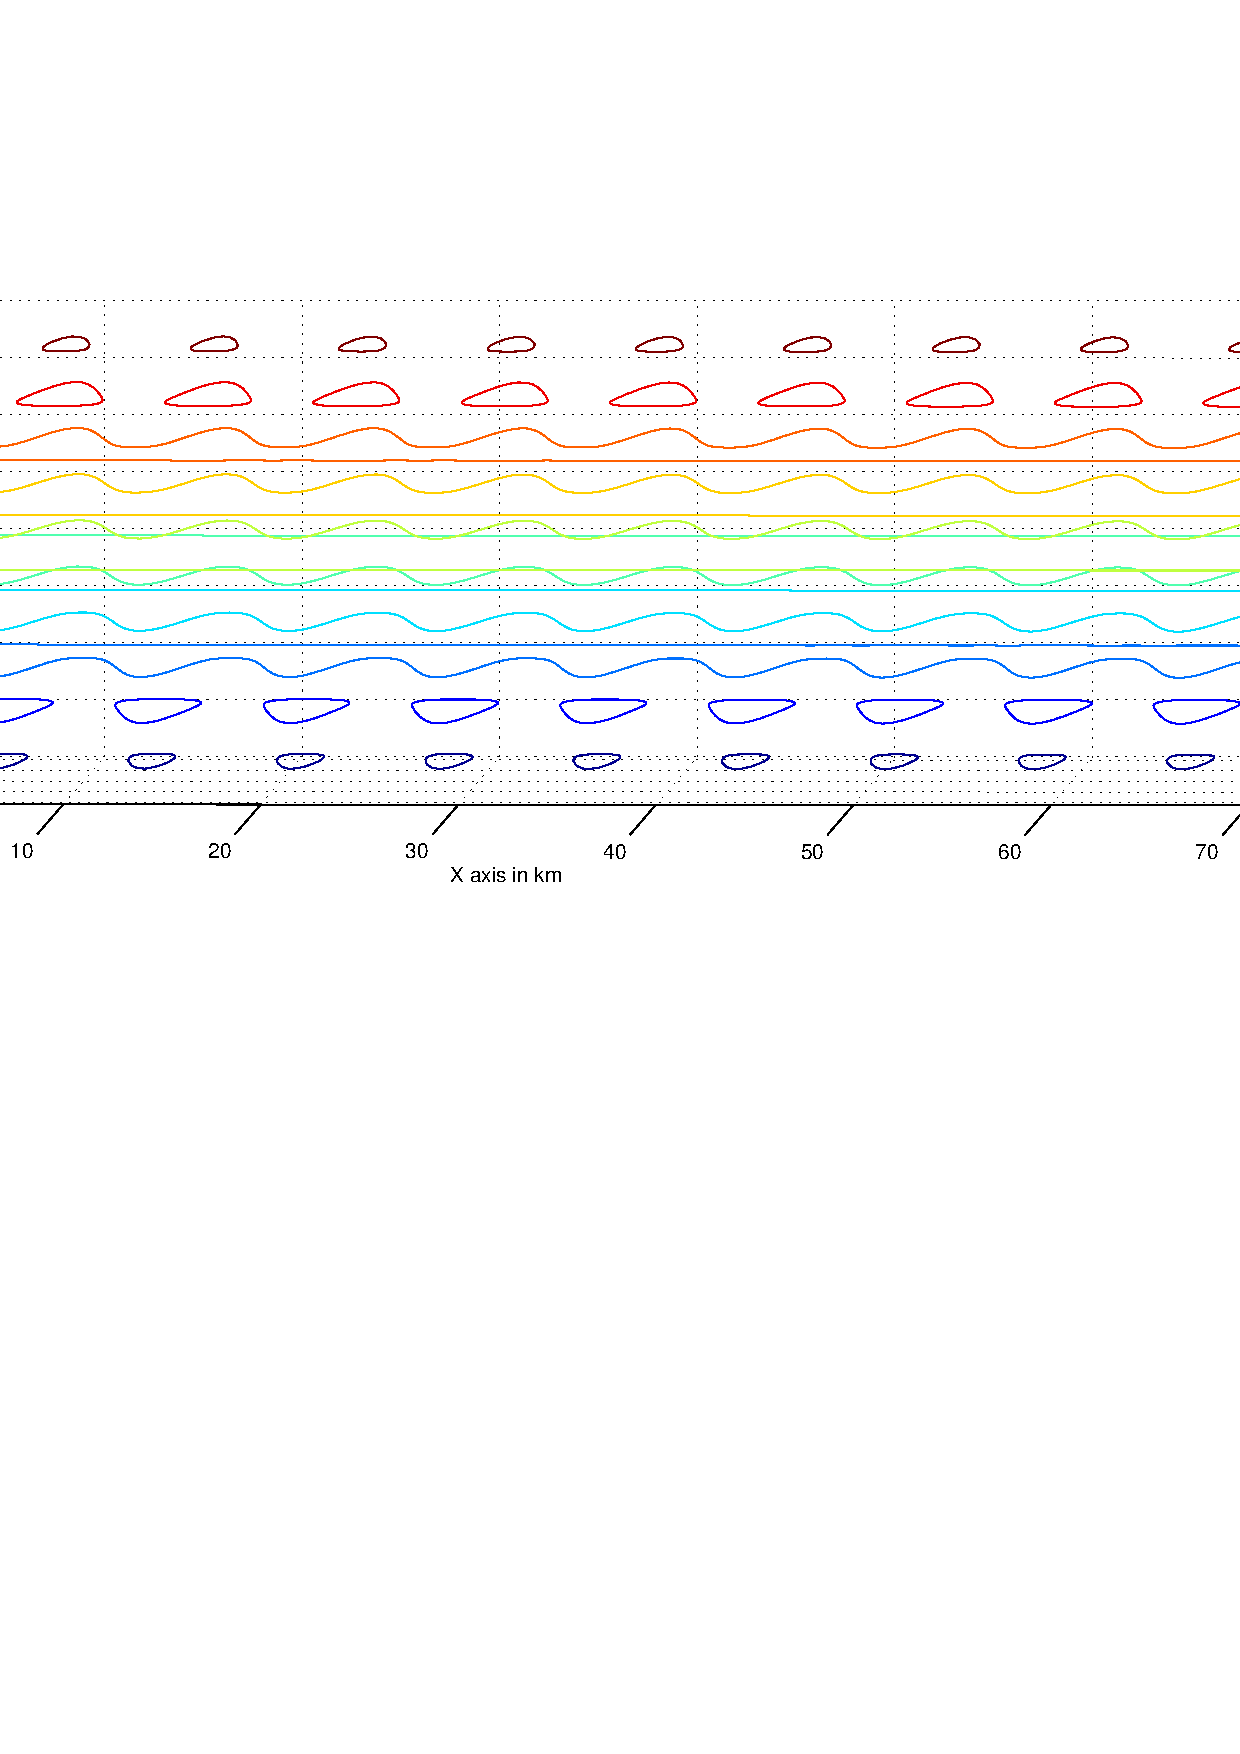
\includegraphics[width=5 in, height=2.5 in]{MCM.pdf}
 \caption{ A plot of stream function \ref{eq:sf} at $t=0$.}
 \label{fig:kme}
\end{figure}

\item Although the above ordinary differential equations are deterministic, small variations in the initial position of a node deployed at t=0 has a strong influence on the trajectory taken by the node (e.g., which circulations it falls into, and for how long).
Figure \ref{fig:res11} illustrates the findings of an experiment where a sample set of 50 nodes are deployed at $t= 0$ in a rectangle of narrow horizontal width at $x=0$, and vertical height in the range $y \in [1.00, 1.30]$ (300 meters). The trajectories are simulated for 2 days. The figure shows the initial positions of the 50 nodes on the left, and the end points of the trajectories at the end of the 2-day period. 
\begin{figure}[!htb]
\begin{minipage}[]{.55\linewidth}
\includegraphics[width=3 in, height=1.8 in]{Endpoints100.pdf}
 \caption{ Start and end points of 50 nodes}
\label{fig:res11}
\end{minipage}
\begin{minipage}{.45\linewidth}
\includegraphics[width=1.8 in, height=2 in,angle=-90]{Endpt.pdf}
 \caption{Probabilistic distribution obtained using a superimposed grid}
\label{fig:ges11}
 \end{minipage}
\end{figure}
\item The above type of simulation experiments can be used to derive the needed probabilities in our probabilistic locality model. For example, as done in figure \ref{fig:ges11}, one can superimpose a grid over the area encapsulating the end points of the 50 trajectories (i.e., the rectangle where $x \in$ [14 Km, 30 Km], and $y \in$ [$-3$ Km, $+2.2$ km]), we then can derive the probability that a node lands in a particular rectangle, say $R$, by dividing the number of end points landed in $R$ over the sample size (50 in this case).
\end{enumerate}
%------------------------------------


%In the next sections we outline the network model and problem formulations.

\section{Network Model}
\label{sec:Nmpf}
In this section, we introduce the concept of \textit{probabilistic graphs} used throughout the thesis. This concept is used to capture node location uncertainty common to UWSNs.

\subsection{Node Locality Sets}
\label{ch1:nls}
We consider UWSNs utilizing both sensor nodes and relay nodes. Sensor nodes can perform sensing, data storage, processing, and communication tasks. Relay nodes can perform data storage and communication only. Several studies on various types of networks have shown that relay nodes can save energy and enhance overall network performance.
We denote by $V=V_{sense}\cup V_{relay}$ the set of nodes in a given UWSN where $V_{sense}$ denotes sensor nodes, and $V_{relay}$ denotes relay nodes.
%
We assume that $V_{sense}$ has a distinguished {\em sink} node,
denoted $s$, that performs network wide command and control functions.


After some time interval $T$ from network deployment time,
each node $x$ can be in some location determined by water currents
causing node movement.


To simplify analysis, current approaches in the literature typically divide
the geographic area containing nodes into rectangles of a superimposed
grid layout.
%
Thus, at time $T,$ each node $x$ can be in any one of a possible
set of grid rectangles denoted $\loc(x)= \{ x[1], x[2], \ldots \}$.
%
We call $\loc(x)$ the {\em locality} set of $x$ (for simplicity,
we omit the dependency on $T$ from the notation).
%
Depending on the mobility model induced by water currents, node $x$
can be in any possible grid rectangle $x[i]$ with a certain probability,
denoted $p_x(i)$. 
%

As mentioned in Section \ref{ch1:wounmm}, one may utilize the kinematic model adopted in \cite{caruso2008meandering} to compute such probabilities from a sufficiently large number of node trajectories simulated by the model.

Henceforth, we use $x[i]$ to refer to node $x$ at the $i^{th}$ location index.
%
For brevity, we also refer to $x[i]$ as the location of $x$
(rather than the grid rectangle containing $x$) at an instant of interest.
%
To gain efficiency in solving large problem instances with large locality
sets, it may be convenient to truncate some locality sets to include only
locations of high occurrence probability, and ignore the remaining locations.
%
In such cases, we get $\sum_{x[i] \in \loc(x)} p_x(i) \leq 1$, if $\loc(x)$
is truncated.

% -------------------------

\subsection{Node Reachability}

At any instant, node $x$ can reach node $y$ if the acoustic signal strength
from $x$ to $y$ (and vice versa) exceeds a certain threshold value.
%
In acoustic UWSN, direction of water currents play an important role
in signal delay (see, e.g., \cite{pu2013comparing}).
%
For simplicity, we assume that given the exact locations of $x$ and $y$, say $x$ at location $x[i]$ and $y$ at location $y[j]$, we can determine if $x$ and $y$ can reach each other, and if so, we
set the link indicator $E_G (x[i],y[j])= 1$.
%
Else, if no satisfactory communication can take place then
we set $E_G (x[i],y[j])= 0$.


Our general objective in this thesis is to develop effective methodologies
for computing lower bounds on the likelihood that the network is totally,
or partially, connected.
%
To this end, we adopt the following rule: we set $E_G(x[i],y[j])= 1$
if and only if the two nodes $x$ and $y$ can reach each other if
they are located anywhere in their respective rectangles $x[i]$ and $y[j]$.


The above rule implies that connectivity between $x$ and $y$ is ignored if 
they can reach each other at some (but not all) pairs of points in their
respective rectangles.
%
As can be seen, ignoring connectivity in such cases results
in computing lower bounds on the network connectivity, as required.
%
Thus we model an UWSN by a probabilistic graph $G=(V=V_{sense}\cup V_{relay},E_G,Loc,p)$.

\section{Problem Formulation}
\label{ch1:pf}
In this section we formulate four probabilistic connectivity problems that we investigate in the thesis. 


\begin{definition}[\textbf{the $A$-$CONN$ problem}]
\normalfont
Given a probabilistic network $G$ with no relay nodes, compute the probability $Conn(G)$ that the network is in a state where the sink node $s$ can reach all sensor nodes. $\blacksquare$
\end{definition}


\begin{definition}[\textbf{the $AR$-$CONN$ problem}]
\normalfont
Given a probabilistic network $G$ where $V_{relay}$ is possibly non-empty, compute the probability $Conn(G)$ that the network is in a state where the sink node $s$ can reach all sensor nodes. $\blacksquare$
\end{definition}


\begin{definition}[\textbf{the $S$-$CONN$ problem}]
Given a probabilistic network $G$ with no relay nodes, and a required number of sensor nodes $n_{req}\leq |V_{sense}|$, compute the probability $Conn(G,n_{req})$ that the network is in a state where the sink node $s$ can reach a subset of sensor nodes having at least $n_{req}$ sensor nodes. $\blacksquare$
\end{definition}


\begin{definition}[\textbf{the $SR$-$CONN$ problem}]

Given a probabilistic network $G$ where $V_{relay}$ is possibly non-empty, and a required number of sensor nodes $n_{req}\leq |V_{sense}|$, compute the probability $Conn(G,n_{req})$ that the network is in a state where the sink node $s$ can reach a subset of sensor nodes having at least $n_{req}$ sensor nodes. $\blacksquare$
\end{definition}

We note some of the above problems are special cases of other problems. Using the polynomial time reducibility relation \cite{cormen2001introduction} denoted $\leq_p$, one can state the following:
\begin{itemize}
\item $\ACONN \leq_p \ARCONN$ and $\SCONN \leq_p \SRCONN$ (since $V_{relay}$ can be an empty set)
\item $\ACONN \leq_p \SCONN$, since $n_{req}$ can be set to $|V_{sense}|$.
\end{itemize}

We next remark that the above problems share some basic aspects with the class of network reliability problems discussed in \cite{Co87}. In particular, all such problems are defined over some type of probabilistic graphs. For network reliability problems, a node or link can either be operating or failed with some known probability, whereas in our present context, a node can be in any one of a possible set of locations with known probability distribution.

Events of interest on such probabilistic graphs occur when the given network is in some particular network states. In our present context, a \textbf{network state} $S$ of $G$ arises when each node $x \in V$ is located at some specific location in its respective locality set $Loc(x)$.
Thus, if $V = \{v_1 , v_2 , . . . , v_n \}$ then a state $S$ of $G$ can be specified by $\{v_1[i_1], v_2[i_2], . . . , v_n[i_n]\}$ where each $v_\alpha[i_\alpha] \in Loc(v_{\alpha})$. Two states $S_1$ and $S_2$ are different if they differ in the location of at least one node. Assuming node locations are independent of each other, we have $Pr(S) =\prod_{v_{\alpha}\in V} p_{v_\alpha[i_\alpha]}$.

{\bf Note:} For a node $v_{\alpha}\in V$ and a possible index $i_\alpha$ in the locality set of $v_{\alpha}$, our use of the notation $v_{\alpha}[i_{\alpha}]$ is overloaded. In some sentences, $v_{\alpha}[i_{\alpha}]$ refers to a particular rectangle in $Loc(v_{\alpha})$. In other sentences, $v_{\alpha}[i_{\alpha}]$ refers to node $v_{\alpha}$ when it is in the location indexed by $i_{\alpha}$ in its locality set. 


In the $A$-$CONN$ and $AR$-$CONN$ problem, a state is \textbf{operating} if the
sink $s$ can reach all sensor nodes in $V_{sense}$ . Likewise, in
the $S$-$CONN$ and $SR$-$CONN$ problem, a state $S$ is \textbf{operating} if the sink node $s$ can reach a subset having at least $n_{req}$ sensor
nodes. Let $\textbf{S}$ be the set of all operating states $S$ of a
given problem. Then the required solution is given by
$\sum_{S\in \textbf{S}} Pr(S)$.

\begin{example}
\normalfont
Figure \ref{fig:Exmp1} illustrates a probabilistic graph on 4 nodes where $V=\{s,a,b,c\}$ and the locality set of each node has 2 locations. The network has $2^4$ states. For the $A$-$CONN$ problem, state $S_1= \{ s[2], a[2], b[2], c[2] \}$ is operating, and
     state $S_2= \{ s[1], a[1], b[1], c[2] \}$ is failed. $\blacksquare$
\end{example}
\begin{figure}[h]
\centering
\includegraphics[width=3.5 in, height=1.8 in]{Figure1.pdf}
 \caption{ An example probabilistic network}
 \label{fig:Exmp1}
\end{figure}

\textbf{The Underlying Graph of Probabilistic Network.} Given a probabilistic network $G=(V,E_G,Loc,p)$ the \textit{underlying graph} of $G$ is an undirected graph $\tilde{G}$ where

\begin{enumerate}[noitemsep]
\item $V(\tilde{G})=V$.
\item $E(\tilde{G})$ has an edge $e=(x,y)$ if for some positions $x[i]$ and $y[j]$ of nodes $x$ and $y$, respectively, we have $E_G(x[i],y[j])=1$.
\end{enumerate}


\begin{example}
\normalfont
The underlying graph of the probabilistic network in figure \ref{fig:Exmp1} is the cycle $(s,a,c,b)$. $\blacksquare$
\end{example}

Equivalently, we say that the probabilistic network $G$ has the topology of the graph $\tilde{G}$. Throughout the thesis, we use the same symbol $G$ to refer to both a probabilistic network and its underlying graph. Overloading the use of the symbol $G$ does not cause confusion since the exact meaning can be deduced by context.
\section{Thesis Organization and Contribution}
\label{sec:thc}

The main research direction undertaken in the thesis is to develop efficient algorithms for handling the defined probabilistic connectivity problems on networks whose underlying graphs have some useful structure. The availability of such algorithms can be used to derive lower bounds on the probabilistic connectivity of any given arbitrary probabilistic network. This approach relies on identifying subgraphs with the desired structure in the graph underlying a given probabilistic network then solving a problem of interest on the identified subgraph.
The thesis pursues this general approach on the well known classes of partial $k$-trees, explained in Chapter 2. The remaining part of the thesis is organized as follows.
\begin{enumerate}
\item Chapter 2 is dedicated to reviewing basic definitions, properties, and algorithmic aspects of $k$-trees and partial $k$-trees.

\item Chapter 3 presents the first contribution of the thesis: an efficient dynamic programming algorithm to solve the $\SRCONN$ problem on probabilistic networks whose underlying graphs are trees. The algorithm solves the more restricted $\ARCONN$ problem with little overhead compared to a dedicated algorithm to solve the $\ARCONN$ problem.
\item Chapter 4 presents a second contribution of the thesis: a dynamic programming algorithm to solve the $\ACONN$ problem on partial $k$-trees. The algorithm runs in polynomial time for any fixed $k$.
\item Chapter 5 considers UWSNs with relay nodes. The chapter presents a third contribution: two dynamic programming algorithms to solve the $\ARCONN$ and $\SRCONN$ problems on partial $k$-trees. The algorithm runs in polynomial time for any fixed $k$. 
\end{enumerate}
Finally Chapter 6 concludes with remarks and possible future research directions

\section{Concluding Remarks}
\label{sec:cg1sum}
In this chapter, we have introduced the notion of a probabilistic network that captures node location uncertainty commonly encountered in UWSNs. Using the notion of probabilistic networks, we have formalized 4 concrete probabilistic connectivity problems whose solution can significantly benefit the design of UWSNs utilizing relay nodes. In the next chapter, we introduce the class of partial $k$-tree that enable the computation of lower bounds on the probabilistic connectivity problems of interest.

\chapter{Algorithmic Aspects of k-Trees}

\begin{quotation}
In this chapter, we review basic definitions and properties of a hierarchy of graph classes known as $k$-trees, where $k\geq 1$. Several important classes of graphs are known to be special cases of partial $k$-trees, for $k=1,2,3$, and $4$. Also, several NP-complete problems have been shown to admit polynomial time algorithms on partial $k$-trees, when $k$ is fixed. Our main contributions in the next chapters show that the probabilistic connectivity problems introduced in Chapter 1 also admit similar polynomial time algorithms. As an introduction to the algorithmic ideas used in subsequent chapters, we review an algorithm due to \cite{wald1983steiner} for solving the Steiner tree problem on partial 2-trees. We conclude by discussing known results on extracting a partial $k$-tree subgraph, with prescribed $k$, from an arbitrary given network.
\end{quotation}

\section{Graph Notation}
\label{sec:graphNotation}

In this section, we introduce a few graph theoretic notations that we need throughout the thesis. In general, we adopt the same notation used, for example, in \cite{cormen2001introduction} and other books. 
An undirected graph $G=(V,E)$ has a set $V$ of \textit{nodes} (or vertices), and a set $E$ of \textit{edges} (or links).
We also use $V(G)$ and $V_G$ to denote the set of nodes. Likewise, we use $E(G)$ and $E_G$ to denote the set of edges. \\
We also need the following notation.
\begin{itemize}[noitemsep]
\item $deg_G(v)$: the degree of node $v$ in graph $G$
\item $N_G(v)$: the set of neighbouring nodes of $v$ in $G$
\item An \textit{induced subgraph} $G'\subseteq G$ on a set $V'\subseteq V$ of nodes contains all edges of $G$ where the two end nodes of each edge lie in $V'$.
\item A clique is a complete graph, and a $k$-clique is a clique on $k$ nodes.
\item A separator in $G$ is a subset of nodes whose removal disconnects $G$ into two, or more, connected components.
\end{itemize}


\section{$k$-Trees and Partial $k$-Trees}
\label{sec:ktree}
{\bf $k$-Trees.} The formulation of $k$-trees dates back to the work of \cite{beineke1969number, beineke1968enumeration} as a generalization of conventional trees. A recursive definition is given below.
\begin{definition} For a given integer $k\geq 1$, the class of $k$-trees is defined as follows
\begin{enumerate}[noitemsep]
\item A $k$-clique is a $k$-tree.
\item If $G_n$ is a $k$-tree on $n$ nodes then so is the graph $G_{n+1}$ obtained by adding a new node, and making it adjacent to every node in $k$-clique of $G_n$. $\blacksquare$
\end{enumerate}
\end{definition}

Thus, trees are 1-trees. A \textit{$k$-leaf} of a $k$-tree $G$ on $k+1$, or more, nodes is a node whose neighbours induce a $k$-clique. By repeatedly deleting $k$-leaves form a $k$-tree $G_n$, on $n\ge k$ nodes, one can reduce $G_n$ to a $k$-clique. We call such a sequence of nodes a \textit{$k$-leaf elimination sequence}.
\begin{example}
\normalfont
Figure \ref{fig:f3t1} illustrates a fragment of $3$-tree $G$ on $n=6$ nodes. $G$ has a $3$-leave $v_b$. $\blacksquare$
\end{example}
\begin{figure}[!htb]
\centering
\includegraphics[width=2.4 in, height=1.5 in]{Ch3f2.pdf}
 \caption{ A fragment of a 3-tree}
 \label{fig:f3t1}
\end{figure}

 The following are basic properties of $k$-trees (for other properties, see e.g., \cite{golumbic2004algorithmic} and \cite{proskurowski1984separating})

\begin{lemma}\label{lem:1} \mbox{ }
\normalfont
\begin{enumerate}[noitemsep]
\item Every $k$-tree that is not a complete graph has at least two non-adjacent $k$-leaves.
\item Given a $k$-tree $G$ and a $k$-clique subgraph $H$ of $G$, there exists a $k$-leaf elimination sequence that reduces $G$ to $H$.
\item Given two non-adjacent nodes $u$ and $v$ of a $k$-tree $G$, a subgraph induced on any minimal $(u,v)$-separator is a $k$-clique. $\blacksquare$
\end{enumerate}
\end{lemma}

{\bf Partial $k$-Trees.} A partial $k$-tree is a $k$-tree possibly missing some edges. The classes of partial $k$-trees, for $k=1,2,3,\ldots$, form a hierarchy of graphs since any partial $k$-tree is also a partial $k+1$-tree. A \textit{leaf} of a partial $k$-tree $G$ is a node $x$ that is a $k$-leaf in some embedding of $G$ in a $k$-tree $\tilde{G}$ (thus, $deg_G(x)\leq k$). A \textit{perfect elimination} of a node $x$ from $G$ is the elimination of $x$ and its incident edges and the addition of the necessary edges to complete $N_G(x)$ to a clique. A \textit{$k$-perfect elimination sequence} $(k\mbox{-}PES)$ of a graph $G$ is an ordering $(v_1,v_2,\ldots,v_r)$ of $V(G)$ such that

\begin{enumerate}[noitemsep]
\item $deg_G(v_1)\leq k$, and
\item for $i=2,3,\ldots,$ the degree of $v_i$ is obtained by removing the sequence $v_1,\ldots,v_{i-1}$ is at most $k$.
\end{enumerate}

\begin{example}
\normalfont 
For the graph $G$ in figure \ref{fig:f3t2}, $(v_a,v_b,v_i,v_j,v_k,v_l)$ is a 3-$PES$. $\blacksquare$
\end{example}
\begin{figure}[!htb]
\centering
\includegraphics[width=2.4 in, height=1.5 in]{Ch2f2.pdf}
 \caption{ A partial 3-tree}
 \label{fig:f3t2}

\end{figure}
Every partial $k$-tree $G$ has a $k\mbox{-}PES$. Similar to Lemma \ref{lem:1} (1), every partial $k$-tree that is not a complete graph has at least two non-adjacent leaves. In Chapters 4 and 5, $G$ is a partial $k$-tree, for some $k$, of some sensor network that contains a sink node $s$. In any completion of $G$ to a $k$-tree $\tilde{G}$, the sink node appears in some $k$-clique $H$. By lemma \ref{lem:1}, one can find a $k$-$PES$ such that the sink node is the last node in the sequence. We henceforth deal with such $k$-$PES$.\\

{\bf Graphs with Bounded Tree-width.}
The work in \cite{robertson1986graph} has introduced the concept of graphs with bounded \textit{tree-width} in the context of resolving a particular graph theoretic conjecture. The concept is defined as follows.
\begin{definition}\normalfont \cite{robertson1986graph}
A \textit{tree-decomposition} of a graph $G$ is a family ($X_i:i\in I$) of subsets of $V(G)$, together with a tree $T$ with $V(T)=I$, with the following properties.
\begin{enumerate}[noitemsep]
\item $\displaystyle \bigcup_{i\in I} X_i =V(G)$.
\item Every edge of $G$ has both its ends in some $X_i$.
\item For $i,j,k \in I$, if $j$ lies on the path of $T$ from $i$ to $k$ then $X_i\cap X_k \subseteq X_j$. $\blacksquare$
\end{enumerate} 
\end{definition}

\begin{definition}
\normalfont
The \textit{width} of a tree-decomposition is $max(|X_i|-1:i\in I)$. $\blacksquare$
\end{definition}
\begin{definition}
\normalfont
The \textit{tree-width} of $G$ is the minimum $w \geq 0$ such that $G$ has a tree-decomposition of width $\leq w$. $\blacksquare$
\end{definition}

\begin{example}
\normalfont
Figure \ref{fig:GandT}(a) illustrates a graph $G$ having a tree-decomposition shown in figure \ref{fig:GandT}(b). The width of the tree decomposition is 3. One may verify that 3 is actually the tree-width of $G$. $\blacksquare$
\end{example}
\begin{figure}[!htb]
\centering
\includegraphics[width=5 in, height=2.2 in]{Ch2f3.pdf}
 \caption{ Tree decomposition}
 \label{fig:GandT}

\end{figure}
The following result is mentioned in \cite{brandstadt1999graph}.
\begin{theorem}
\normalfont
$G$ has tree-width $\leq k$, if and only if $G$ is a partial $k$-tree. $\blacksquare$ 
\end{theorem}

{\bf Relation to Other Graph Classes:}  Several classes of graphs surveyed in \cite{brandstadt1999graph} are known to be partial $k$-trees for fixed $k$. For example, 
\begin{itemize}[noitemsep]
\item  Cactus graphs, series-parallel graphs, and outerplanar graphs are partial 2-trees.
\item Halin graphs and Y-$\Delta$ graphs are partial 3-trees.
\item A chordal graph $G$ with maximum clique of $\omega (G)$  nodes is a  partial $(\omega (G)-1)$-tree. A graph is chordal if it has no induced cycle on 4 or more nodes.
\item An $n\times n$ grid (on $n^2$ nodes), $n\geq 2$, has tree-width $n$.
\end{itemize}
\section{Dynamic Programming on Partial $k$-Trees}
\label{ch2:dpk}
The theory of partial $k$-trees and graphs with bounded tree-width is rich with dynamic programming algorithms for solving many problems that are NP-complete in general.
The work of \cite{arnborg1989linear} is an example survey paper of such algorithm published in or before 1989.
%
More recently, there has been work on obtaining unifying results that show classes of problems that admit polynomial time solutions on partial $k$-trees, for fixed $k$.
%
Example of such unifying results include the work of \cite{bodlander1988} and \cite{arnborg1991easy}.

The approach used in such results relies on formalizing graph and network properties as logical statements in a particular logic system. 
Such approaches are not intended to provide optimized algorithms for solving any particular problem at hand, or implementing a direct solution. It is often more fruitful to construct a direct algorithm for handling a given problem of interest.
In the rest of the section, we review a dynamic programming algorithm result due to \cite{wald1983steiner} for solving the Steiner tree problem on partial 2-trees.
This dynamic programming algorithm has inspired the design of many subsequent algorithms for solving other NP-complete problems on partial $k$-trees. 
A Steiner tree can be defined as follows.
\begin{definition}
\normalfont
Given a graph $G = (V,E)$ with positive integer edge costs, and a set of target nodes $V_{target}\subseteq V$, a Steiner tree, denoted $ST(G,V_{target} )$, is a subtree $G' = (V',E')$ satisfying
\begin{enumerate}[noitemsep]
\item  $V_{target} \subseteq V'\subseteq V$ ,
\item the sum of edge costs in $E'$ is minimum over all subtrees satisfying (1). $\blacksquare$
\end{enumerate}
\end{definition}

The algorithm devised in \cite{wald1983steiner} works as follows. The graph is reduced by repeated deletion of degree-2 vertices until the graph which remains is a single edge. During this vertex elimination procedure, the algorithm summarize information about the triangle
$\{ x , y , z \}$ , where $y$ has degree 2, on the arcs $(x,z)$ and $( z , x )$ , prior to deleting $y$. This
summary information encodes information about Steiner trees in the subgraph of the 2-tree which has thus far been reduced onto the edge $\{x, z \}$. With each edge $\alpha = (x, y)$ of $G$, the algorithm associates six cost measures, which summarize the cost incurred so far of the subgraph $S$ which has been reduced onto the edge $(x , y )$ \cite{wald1983steiner}:
\begin{enumerate}[noitemsep]
\item $st(\alpha)$ is the minimum cost of a Steiner tree for $S$, in which $x$ and $y$ appear in the same tree.
\item $dt(\alpha)$ is the minimum cost of two disjoint trees for $S$ including all targets, one tree involving $x$ and the other $y$.
\item  $yn(\alpha)$ is the minimum cost of a Steiner tree for $S$, which includes $x$ but not $y$.
\item $ny(\alpha)$ is the minimum cost of a Steiner tree for $S$, which includes $y$ but not $x$.
\item $nn(\alpha)$ is the minimum cost of a Steiner tree for $S$, which includes neither $x$ nor $y$.
\item $none(\alpha)$ is the cost of omitting all vertices of $S$ from a Steiner tree.
\end{enumerate}
The six measures are initialized as follows:
\begin{enumerate}[noitemsep] 
\item $st(\alpha)=cost(\alpha)$
\item $dt(\alpha)=0$
\item  $yn(\alpha)=BIG$ if $y\in V_{target},0$ otherwise.
\item $ny(\alpha)=BIG$ if $x\in V_{target},0$ otherwise.
\item $nn(\alpha)=BIG$ if $x\in V_{target}$ or $y\in V_{target},0$ otherwise.
\item $none(\alpha)$ if $x\in V_{target}$ or $y\in V_{target},0$ otherwise.
\end{enumerate}
A cost of $BIG$ is incurred whenever an attempt is made to omit a target vertex.
The initial edge costs are used to update edge costs as the graph is reduced. The graph is reduced by repeated deletion of degree-2 vertices. So, suppose at some point there is a triangle $\{ x , y , z \}$ in which $y$ is a degree-2 vertex, and valid costs have been computed for $( x , y )$ and $(y,z)$. The algorithm uses these values to update the costs for $( x , z )$ prior to deleting $y$, as follows. Let $L = (x,y)$, $R = (y , z )$, and $M = ( x , z )$. The costs are updated for $M$ using the following recurrences \cite{wald1983steiner}:

\begin{enumerate}[noitemsep]
\item $st(M)=min[st(M)+min[dt(L)+st(R),st(L)+dt(R),yn(L)+ny(R)],dt(M)+st(L)+st(R)]$,
\item $dt(M)=dt(M)+min[dt(L)+st(R),st(L)+dt(R),yn(L)+ny(R)]$,
\item $ny(M)=ny(M)+min[ny(L)+st(R),none(L)+ny(R)]$,
\item $yn(M)=yn(M)+min[yn(L)+none(R),st(L)+yn(R)]$,
\item $nn(M)=min[nn(M)+none(L)+none(R),none(M)+nn(L)+none(R),none(M)+none(L)+nn(R),none(M)+ny(L)+yn(R)]$,
\item $none(M)=none(M)+none(L)+none(R)$,
\end{enumerate}



An alternative approach to present the above algorithm is to store the six measures associated with edge $\alpha=(x,y)$ in a table, denoted $T_{x,y}$. The table provides key-value mappings. Roughly speaking, the keys replace the use of some of the names $st,dt,yn, $ etc. with set notation. Not all names correspond to keys in this formulation. Examples of names that correspond to keys are:

$st=\{x,y\}_1,dt=\{x\}_1\{y\}_1, yn=\{x\}_1\{y\}_0, \mbox{ and } ny=\{x\}_0\{y\}_1$.


As can be seen, each key contains a partition of the set $\{x,y\}$. To explain the keys, let $S$ be a subgraph reduced onto the edge $\alpha=(x,y)$ in some iteration of the algorithm, and let $S'\subseteq S$ be a subgraph of $S$ that is a candidate for appearing in a final solution. We now have:

\begin{itemize}[noitemsep]
\item The key $\{x,y\}_1$ is associated with a minimum cost $S'$ such that both $x$ and $y$ appear in one connected component of $S'$, and this component has at least one target node (counting $x$ and $y$ as possible target nodes). 
\item The key $\{x\}_1\{y\}_0$ is associated with a minimum cost $S'$ such that  $x$ and $y$ appear in two different components of $S'$, and only the component that includes $x$ contains one, or more, target nodes.
\end{itemize}
In this alternative approach, the above recurrences are replaced by functions that merge 3 tables $T_{x,y}, T_{y,z}$ and $T_{x,z}$ into an updated $T_{x,z}$ table.

\section{Set Partitions}
\label{sec:setPartitions}
The dynamic programs devised in the rest of the thesis make heavy use of set partitioning, as explained below. Given a set $X$, a partition of $X$ is a set $\{X_1,X_2,\ldots, X_r\}$, $1\leq r\leq |X|$ such that 
\begin{enumerate}
\item $X=\displaystyle \bigcup_{i=1,2,\ldots,r} X_i$.
\item The $X_i$s are pairwise disjoint.
\end{enumerate}
In our algorithm, $X$ is a set of nodes in a $k$-clique, and the partition of $X$ are used as part of states of dynamic programs.
%
The number of all possible partition of a set $X$ on $n$ elements are known as Bell numbers, denoted $B_n$ (see for example \cite{brualdi2009introduction}).
The first few Bell numbers are 
\begin{center}
$\begin{array}[t]{l}
B_0=B_1=1,B_2=2,\\
B_3=5,B_4=15,B_5=52,\\
B_6=203,B_7=877,B_8=4140, \ldots \\
\end{array}$
\end{center}
Bell numbers satisfy the following recurrence equation:
\begin{center}

$ B_0=1, B_1=1 \mbox{ and } B_{n+1}=\displaystyle \sum_{k=0}^n (\begin{array}{l} n \\ k \end{array})B_k.
$
\end{center}

\section{Finding Good Partial $k$-Tree Subgraphs}
\label{sec:fgpkts}

The algorithms presented in Chapters 3 to 5 can be used to derive lower bounds on the $Conn(G)$ and $Conn(G,n_{req})$ measures. This is done by
\begin{enumerate}
\item  constructing a graph $G$ that underlies the structure of a given probabilistic graph of the problem instance at hand (as explained in subsequent chapters), and
\item  identifying a subgraph $G'$ of $G$ that is a partial $k$-tree, of some user specified $k$.
\end{enumerate}
Under simple assumptions, we have $Conn(G')\leq Conn(G)$ (or, $Conn(G',n_{req})\leq Conn(G,n_{req})$).
So $Conn(G')$, or $Conn(G',n_{req})$, is a lower bound on the required solution.

Ideally, one would prefer to use a subgrpah $G'$ that gives the best possible lower bound. The problem of finding such subgraph is a complex graph problem. This class of problems is related to the following classes of problems.

\begin{enumerate}[noitemsep]
\item {\bf Recognizing  Partial $k$-Trees:} Given a graph $G$, and an integer $k\geq 1$, is $G$ a partial $k$-tree?\\
\begin{itemize}
\item The work of \cite{arnborg1987complexity} shows $O(n^{k+2})$ algorithm for solving the problem. If $k$ is not fixed, then \cite{arnborg1987complexity} shows that the problem is NP-complete.

\item For any fixed  $k$, the work of \cite{bodlaender1993linear} improves on the above result by showing a linear time recognition algorithm.
\end{itemize}
The above results produce also a $k$-$PES$ if one exists.\\

\item {\bf Edge Deletion Problem (EDP) to Obtain a Partial $k$-Tree:}  Given a graph $G$, and an integer $k$, find the minimum number of edges whose deletion gives a partial $k$-tree.
\begin{itemize}
\item For $k=1$, the problem is simple.
\item For $k\geq 2$, the problem is NP-complete (see, e.g. the work of \cite{el1988complexity} and the references therein)
\end{itemize}
\end{enumerate}

In the absence of known algorithms to find the required best subgraphs, we resort to using heuristic algorithms. In Chapters 3 to 5, we experiment with partial $k$-tree subgraphs ($k=1,2, \mbox{ and }3$) obtained using the following methods. We assume that $G$ is a connected graph.


\nwline
{\bf The Random Method.} Subgraphs obtained using the random method are used as baseline cases for comparisons. This method constructs a partial $k$-tree subgraph for $k=1,2, \mbox{ and }3,$ as follows.
\begin{itemize}
\item {\bf Case $k=1$.} Choose any spanning tree.
\item {\bf Case $k=2$.} Choose a spanning tree $G'\subseteq G$. Fix an ordering of the remaining edges not in $G'$. For each edge $e$ in the fixed order, test whether $G'+e$ is a partial 2-tree. If yes, add $e$ to $G'$, and proceed to the next edge in the fixed order.
\item {\bf Case $k=3$.} Build a partial 2-tree $G'\subseteq G$ as in case $k=2$, and let $S=(v_1,v_2, \ldots,v_{n-2})$ be a $2$-$PES$ of $G'$. Fix an ordering of the edges not in $G'$. For each edge $e$ in the fixed order, test whether $G'+e$ is a partial 3-tree with $S$ being a 3-$PES$.  If yes, add $e$ to $G'$, and proceed to the next edge in the fixed order.
\end{itemize}
\nwline
{\bf The Greedy Method.} Here, we associate with each link $(x,y)\in E_G$ a probability, denoted $p(x,y)$, of having the link $(x,y)$ present, given the locality sets $Loc(x)$ and $Loc(y)$. For convenience of using a minimum spanning tree algorithm, we transform each non-zero edge probability $p(x,y)> 0$ into edge cost using the relation $cost(x,y)=-\log p(x,y)$. The greedy method constructs partial $k$-tree subgraphs for $k=1,2,$ and $3$ as follows.
\begin{itemize}
\item {\bf Case $k=1$:} Choose a minimum spanning tree using the above edge costs.
\item {\bf Case $k=2$ and $3$:} As in cases $k=2$ and $3$, respectively, of the random method, where we sort the remaining edges in a non-decreasing order of their costs to obtain the fixed order
\end{itemize}



\section{Concluding Remarks}
\label{ch2:sum}
In this chapter we have presented some background information on $k$-trees and partial $k$-trees that serves as an introduction to the algorithms developed in subsequent chapters. 
\chapter{Probabilistic Connectivity of Tree Networks}
\begin{quote}

In this chapter, we consider the connectivity problems introduced in Chapter 1 on probabilistic graphs that have the topology of a tree. We present a dynamic programming algorithm to solve the $SR$-$CONN$ problem on such networks. The algorithm is designed to solve the more restricted $AR$-$CONN$ problem while incurring only a small overhead compared to a specialized algorithm for solving the problem. Since the $SR$-$CONN$ problem is the most general problem among the four problems defined in Chapter 1, it follows that the algorithm presented in this chapter can solve the remaining three probabilistic connectivity problems. Results in this chapter appear in our work in \cite{Tree2014}.
\end{quote}

\section{System Model}
\label{sec:ch3sm}
We recall that a probabilistic graph $G=(V,E_G,Loc,p)$ is specified by the following:
\begin{itemize}[noitemsep]
\item $V=V_{sense}\cup V_{relay}$ the set of nodes in a given UWSN $G$
\item $E_G(x[i],y[j])=1$ if and only if the two nodes $x$ and $y$ can reach each other when located anywhere in their respective rectangles $x[i]$ and $y[j]$. This restriction results in computing lower bounds on the solution since we ignore cases where $x$ and $y$ can reach each other if they are located in some (but not all) positions in their respective rectangles.
\item $Loc(v)$ is the locality set of node $v$. 
\item $p_v(i)$ is the probability that node $v$ is located at grid rectangle $v[i]$. 
\end{itemize}
We say that the probabilistic graph $G$ has the topology of a conventional tree $T=(V,E_T)$ if whenever $E_G(x[i],y[j])= 1$
then $(x,y) \in E_T$.
%
Note that the definition allows two nodes $x$ and $y$ to be adjacent in
$T$, and yet they can take positions, say $x[i]$ and $y[j]$, such that
$E_G (x[i],y[j])= 0$.
%
Thus, each state $S$ of $G$ gives a subgraph of $T$.\\
\nwline
In any such tree network $T$, one may safely delete a relay node
$x \in V_{relay}$ that appears as a leaf node without changing the problem
solution. 
%
This observation holds since relay nodes are relevant only if they
connect some sensor node to the sink $s$.
%
We henceforth assume, without loss of generality, that the input network $G$ has no relay leaf.\\


We also recall that in the $AR$-$CONN$ problem, a state is {\em operating} if the sink $s$
can reach all sensor nodes in $V_{sense}$.
%
In the $SR$-$CONN$ problem, a state $S$ is {\em operating} if
the sink node $s$ can reach a subset having at least $n_{req}$ sensor nodes.
%
Let $\textbf{S}$ be the set of all operating states $S$ of a given
$AR$-$CONN$ or $SR$-$CONN$ problem then the required solution is given by $\sum_{S \in \textbf{S}} Pr(S)$.
\section{Overview of the Algorithm}
The algorithm (Function $Conn$ in Figure ~\ref{alg:Conn}) employs a
dynamic programming approach.
%
It takes as input an instance $(G,n_{req})$ of the $SR$-$CONN$ problem,
and a tree $T=(V,E_T)$ on the set $V$ of nodes with no relay leaves.
%
The function computes the exact solution $Conn(G,n_{req})$ of the given
instance.

The pseudo-code uses syntax similar to $C/C\mbox{++}$ languages. In particular, we use $x \starEqual y$ (or, $x \plusEqual y$) to mean $x=x*y$ (respectively, $x=x+y$).
We consider $T$ as a tree rooted at the sink $s$. Each node $y$ in $T$ except $s$ has a parent node $x$ on the unique path from $y$ to the root $s$.
%
Each such node $y$ is a root of a subtree, denoted $T_y=(V_y,E_{T_y})$, obtained by
removing the link $(y, parent(y))$ from $T$.

%----------------------------
%There will be a figure here
%---------------------------------
\begin{example}
\normalfont
Figure \ref{fig:es31} illustrates a tree network where $|V_{sense}|=7$ and $|V_{relay}|=3$ nodes. $Children(x_2)=\{y_1,y_2,y_3\}$ and subtree $T_{y_3}$ has nodes $\{y_3,z_3,z_4\} \blacksquare$.
\end{example}
\begin{figure}[!htb]
\centering
\includegraphics[width=3 in, height=1.8 in]{Ch4f1.pdf}
 \caption{ A tree network}
\label{fig:es31}
\end{figure}

The key variables and data structures in the function are as follows.

\begin{itemize}[noitemsep]
\item	$type(x)$:
	For any node $x$, $type(x)= 0$ if $x$ is a relay node,
	and $type(x)= 1$ if $x$ is a sensor node.

\item	$n_{sense}(X)$: The number of sensor nodes in a given subset  of nodes $X\subseteq V$. We use $n_{sense}$ for $n_{sense}(V)$.


\item   $n_{relay}(X)$: The number of relay nodes in a given subset of nodes $X\subseteq V$. We use $n_{relay}$ for $n_{relay}(V)$.

\item $n(X)=n_{sense}(X) + n_{relay}(X)$.

\item $n_{sense,min}(X)$: The minimum number of sensor nodes in a given subset $X\subseteq V$ that should be connected to the sink in any operating state of the overall network. So,\\
\centerline{
$n_{sense,min}(X)=max(0,n_{req}-n_{sense}(\overline{X}))$
}

\nwline
where $\overline{X}=V\setminus X$ (the complement set of $X$). So $n_{sense}(\overline{X})$ is the number of available sensor nodes not in $X$. Consequently, $n_{req}-n_{sense}(\overline{X})$, if non-negative, is the minimum number of sensor nodes of $X$ required in any operating state of the network. 

\begin{example}
\normalfont
In figure \ref{fig:es31}, consider node $x_2$. Using the above notation, $n(V_{x_2})=8$ where $n_{sense}(V_{x_2})=5$ and $n_{relay}(V_{x_2})=3$. Assuming $n_{req}=5$ in an instance of the $\SRCONN$ problem then $n_{sense,min}(V_{x_2})=3=n_{req}-n_{sense}(\{s,x_1\})=5-2$ $\blacksquare$
\end{example}
The dynamic program associates with each node $x$ a table, denoted $R_x$. Initially, $R_x$ contains information derived from node $x$ only. Subsequently, the algorithm performs $n-1$ iterations. Each iteration of the main loop in Step 2 identifies
	a non-sink leaf node $y$ in the current tree whose parent is denoted $x$. 
	The function then processes, and then deletes node $y$. Processing of node $y$ is done by updating summary information in table $R_x$ using information in table $R_y$. Subtree $T_y$ is considered one part of the tree $T_x$ that has been processed thus far. We also need the following definitions and notation.

\item	$DCH(x)$:	In any iteration, each node $x$ may have some of its children
	processed and deleted.
	We denote such set of $x$'s \textbf{deleted children} by $DCH(x)$.

\item	Tables $R_x$ (and $R'_x$):
	Each node $x \in V$ is associated with a table $R_x$.
	The table stores {\em key-value} mappings.
	%
	Each key is a pair $(i,count)$ where $i$ is a possible location
	index of $x$, and $count$ is a number of sensor nodes that are
	descendants of $x$ (including $x$ itself) in the graph processed
	thus far.
	%
	Roughly speaking, at any iteration of the main loop,
	$R_x(i,count)$ is the probability of obtaining a state over
	the subset of nodes in $T_x$ processed in previous iterations
	where $x[i]$ reaches exactly $count$ sensor nodes in such subset of
	$T_x$. 

\end{itemize}
\begin{example}
\normalfont
In figure \ref{fig:es31}, consider node $x_2$ and its associated tree $T_{x_2}$. Assume that the algorithm has processed and deleted nodes in subtree $T_{y_1} \mbox{ and } T_{y_2}$. Thus, $DCH(X)=\{y_1,y_2\}$, and all nodes in $V_{y_1}\cup V_{y_2}=\{z_1,z_2,y_1,y_2\}$ have been deleted. Now assume that $n_{req}=5$. After deleting nodes in  $V_{y_1}\cup V_{y_2}$, the algorithm computes\\
\centerline{
$n_{sense,min}(\{x_2\}\cup V_{y_1}\cup V_{y_2}) \begin{array}[t]{l}
=n_{req}-n_{sense}(\{s,x_1,y_3,z_3,z_4\})\\
=5-4\\
=1
\end{array}
$
}
This value is the minimum number of sensor nodes in the set $X=\{x_2\}\cup V_{y_1}\cup V_{y_2}$ required to be connected to the sink in any operating state of the overall graph. $\blacksquare$
\end{example}
% ------------------------------
    % --------------- Function E2P ---------------
    \begin{figure}[htbp]
    % \begin{figure}[!ht]
    \small
\begin{center}
\fbox{
    \begin{minipage}[t]{6 in}
    \renewcommand{\baselinestretch}{1}
    %
    {\bf Function $\fConn (G, T, \nReq)$}
\nwline
	{\bf Input:}
	\begin{minipage}[t]{5in}
	An instance of the $SR$-$CONN$ problem where $G$ has a tree
	topology $T$ with no relay leaves
	\end{minipage}
%
\nwline
	{\bf Output:}
	\begin{minipage}[t]{5in}
	$Conn(G, \nReq)$
	\end{minipage}
	\\
%
%\nwline
%	{\bf Notation:}
%	\begin{minipage}[t]{2.75in}
%	\end{minipage}
% --------------------
   \nwline
% initialization
   1.  \begin{minipage}[t]{5in}
       {\bf foreach} (node $x$ and a valid location index $i$) \\
       \{ \\
         \iin{0.20} set $R_x(i, type(x) )= 1$ \\
         %\iin{0.20} $n_{x,min}= \min (0, \nReq - (n_{sense} - n_{x,sense}) )$ \\
       \}
       \end{minipage}
       \\
   \nwline       
% main loop
   2.  \begin{minipage}[t]{5in}
       {\bf while} ($T$ has at least 2 nodes) \\
       \{
       \end{minipage}
       \\
   3.  \iin{0.20} \begin{minipage}[t]{5 in}
   		  Let $y$ be a non-sink leaf of $T$, and $x= parent(y)$
		  \end{minipage}
		  \\
   4.  \iin{0.20} \begin{minipage}[t]{5 in}
   		  {\bf foreach} (key $(i,count) \in R_y$)
		       $R_y (i,count) \starEqual p_y(i)$
		  \end{minipage}
		  \\
   5.  \iin{0.20} \begin{minipage}[t]{5in}
   		  set $R'_x= \phi$
		  \end{minipage}
		  \\
   6.  \iin{0.20} \begin{minipage}[t]{5in}
   		  {\bf foreach} (pair of keys
		       		$\begin{array}[t]{l}
				 (i_x, count_x) \in R_x \mbox { and }
		   		 (i_y, count_y) \in R_y)
				 \end{array}
				$ \\ 
		  \{
		  \end{minipage}
		  \\
   7.  \iin{0.40} \begin{minipage}[t]{5 in}
   		  $count= \min (\nReq, count_x + count_y)$
		  \end{minipage}
		  \\
%   8.  \iin{0.40} \begin{minipage}[t]{5 in}
%   		  $count_{x,min}= \begin{array}[t]{l}
%		  		  type(x) + n_{y,min} + 
%		       	   	  \sum_{z \in \DCH(x)} n_{z,min}
%				  \end{array}$
%		  \end{minipage}
%		  \\
  8.  \iin{0.40} \begin{minipage}[t]{5 in}
   		  {\bf if} ($count < n_{sense,min}(\{x\}\cup V_y \cup_{z\in DCH(x)} V_z)$) {\bf continue} 
		  \end{minipage}
		  \\
   9.  \iin{0.35} \begin{minipage}[t]{5in}
   		  $R'_x (i_x,count) \plusEqual$ 
		  	$\begin{array}[t]{l}
			 R_y(i_y,count_y) \times 
			 R_x(i_x,count_x) \times 
			 E_G(x[i_x], y[i_y])
		  	 \end{array}$
		  \end{minipage}
		  \\
       \iin{0.40} \} \\
   10. \iin{0.20} \begin{minipage}[t]{5 in}
       		  set $R_x= R'_x$; remove $y$ from $T$
		   \end{minipage}
		   \\
       \iin{0.15} \} \\
   11. \begin{minipage}[t]{6 in}
       return $\sum_{s[i] \in \loc(s)} R_s(i,\nReq) * p_s(i)$
       \end{minipage}
       \\
    \end{minipage}	
}
\end{center}
    \normalsize
    %
    \caption{Pseudo-code for function $\fConn$}
    \label{alg:Conn}
\vspace*{-0.1in}
    \end{figure}
    % ------------------------------
\section{Main Steps}
Step 1 initializes table $R_x$ for each node $x$ as follows.
%
For each possible location index $i$ of $x$, set $R_x(i, count=1)= 1$
if $x$ is a sensor node.
Else ($x$ is a relay node), set $R_x(i, count=0)= 1$.
%
%Step 1 also initializes $n_{x,min}$.


Steps 2-10 form the main loop of the function.
The loop iteratively finds a leaf node $y$ that is not the sink $s$, 
processes node $y$, and then removes $y$ from the tree $T$.
%
Processing a node $y$ with parent $x$ is done as follows.

Step 4 updates each entry $R_y (i,count)$ by multiplying the entry
with $p_y(i)$.
%
As can be seen, this update operation is done in the iteration that ends by
removing $y$.
%
Step 5 initializes the temporary table $R'_x$ to empty.


Steps 6-9: the loop in Step 6 performs a {\em cross product} of tables
$R_x$ and $R_y$, storing the result in table $R'_x$.
%
In the cross product, each pair of possible keys $(i_x, count_x)$
and $(i_y, count_y)$ are processed.
%
More specifically, suppose that $x[i_x]$ can reach $count_x$ sensor nodes
in the part of $T_x$ processed thus far with probability $R_x(i_x,count_x)$.
%
Also, suppose that $y[i_y]$ can reach $count_y$ sensor nodes
in $T_y$ with probability $R_y(i_y,count_y)$.
%
Thus, if $x[i_x]$ reaches $y[i_y]$ (i.e., $E_G(x[i_x],y[i_y])$= 1)
then $x[i_x]$ can reach a total of $count= count_x + count_y$ nodes.


If $count > \nReq$ then Step 7 truncates $count$ to $\nReq$.
%
On the other hand, if $count < n_{sense,min}(\{x\}\cup V_y  \cup_{z\in DCH(x)} V_z)$ (i.e., $count$ is below the
minimum number of nodes required to construct an operating state) then
Step 8 skips Step 9 and starts a new iteration.
%
Step 9 updates the probabilities accumulated in $R'_x(i_x,count)$. 


After exiting the main loop, the current tree $T$ contains only the
sink node $s$. Step 11 computes the solution $Conn(G,\nReq)$ from
the table $R_s$ associated with the sink $s$.
% ------------------------------

\section{Correctness}

To prove correctness, we first introduce the following notation and
definitions.
%
For a given node $x$, and iteration $r \in [1,n-1]$ of the main loop
in Step 2, we have the following:
%
\begin{itemize}
\item	$\DCH (x,r)$:
	The set of $x$'s deleted children at the start of iteration $r$.

\item	$V_{x,deleted,r}$ ($= \bigcup_{y \in \DCH(x,r)} V_y$):
	The set of $x$'s deleted descendants at the start of iteration $r$.
\end{itemize}
%
For brevity, we omit $r$ when the iteration number is not important, or
understood by the context.


In the following definitions, $x$ is any node in $T$,
$i$ is a possible location index of $x$, and  $V_{x,delete}$ is
the set of deleted descendants associated with $x$ at the start of some
iteration.

\begin{enumerate}[noitemsep]
\item[{\bf [D1]}]
    Let $S$ be a state over nodes in $\{ x \} \bigcup V_{x,delete}$.
    The {\em type} of $S$ is a pair $(i,count)$ where
    %
    \begin{itemize}
    \item   $x$ is at location $x[i]$
    \item   If $count = \nReq$ then the number of sensor nodes connected to
    	    $x[i]$ in $S$ is $\geq \nReq$
    \item   Else ($count < \nReq$), then the number of sensor nodes
    	    connected to $x[i]$ is $< \nReq$
    \end{itemize} 	   
\end{enumerate}

\begin{enumerate}
\item[{\bf [D2]}]
    We say that table $R_x$ is {\em complete} with respect to a given
    set $V_{x,delete}$ if the following conditions hold:
    %
    \begin{enumerate}
    \item  For each key $(i,count)$ in $R_x$, $R_x(i,count)$ is
    	   the probability of obtaining states over
	   $\{ x[i] \} \bigcup V_{x,delete}$ of type $(i,count)$.
	   (Before multiplying by $p_x(i)$, the probability is conditioned
	   on $x$ being at location $x[i]$).
    \item  Each key $(i,count)$ not in $R_x$ does not contribute to
    	   computing the solution $Conn(G,\nReq)$.
    \end{enumerate}
\end{enumerate}

\nwline
We now show the following theorem.

\begin{theorem} \label{thm:correctness}
\normalfont
    At the start of each iteration of the main loop in Step 2,
    if $x$ is a node in the current tree $T$ then table $R_x$ is complete
    with respect to the associated set $V_{x,delete}$ of deleted nodes.
\end{theorem}

\nwline
{\bf Proof.}
\nwline
{\bf Loop initialization:}
At the start of the 1st iteration, $T$ contains all nodes $V$, and
each node $x$ has $V_{x,delete}= \emptyset$.
%
Node $x$ in location $x[i_x]$ is associated with one state of type
$(i_x,count_x= 0)$ if $x$ is a relay node, or type
$(i_x,count_x= 1)$ if $x$ is a sensor node.
%
For each such state type, Step 1 correctly sets $R_x(i,count)$.

\nwline
{\bf Loop maintenance:}
Assume the theorem holds for all possible iterations $r$, where $r \leq n-2$.
We show that it holds in iteration $r+1$.
%
Let $y$ be the leaf node deleted in iteration $r$, and $x= parent(y)$.
$R_x$ is the only relevant table that may have changed between iterations
$r$ and $r+1$ (table $R_y$ is also changed but node $y$ is deleted at the end of the iteration).
%
Thus, it suffices to show that $R_x$ is complete with respect to
$\{ x \} \bigcup V_{x,delete,r+1}$ at the start of iteration $r+1$.
%
To this end, we note the following in iteration $r$:
%
\begin{itemize}[noitemsep]
\item  Step 4: this step adjusts the probability of each state type
       $(i,count)$ in $R_y$ by taking into account $p_y(i)$.
\item  Step 6: this loop exhaustively generates all state types over the
       set $V_y \bigcup V_{x,delete,r}$ where $V_y$ is all nodes of
       the subtree rooted at node $y$.
\item  Step 8: this step discards all state types that can not be extended
       (by adding sensor nodes from the unprocessed part of the tree)
       to satisfy the $\nReq$ requirement.
\item  Step 9: this step updates the probability of $R'_x(i_x,count)$ by
       adding the right hand side when states of type $(i_x, count)$
       can be extended to operating states.
\end{itemize}
$\blacksquare$

Following an argument similar to the loop maintenance argument, one can
show that at Step 11, table $R_s$ associated with the sink node is
complete with respect to all nodes $V$ in the network.
%
Thus, the function returns the required solution $Conn(G, \nReq)$.

% ------------------------------

\section{Running Time}

Let $n$ be the number of nodes in $G$, and $\ell_{max}$ be the maximum
number of locations in the locality set of any node.

% ----------
\begin{theorem}
\normalfont
    Function $\fConn$ solves the $\SRCONN$ problem in
    $O(n \cdot n_{req}^2  \cdot \ell_{max}^2)$ time
\end{theorem}

\nwline
{\bf Proof.}
We note the following.
\begin{itemize}[noitemsep]
\item   Step 1: storing the tree $T$ requires $O(n)$ time.

\item	Step 2: the main loop performs $n-1$ iterations.
	Each of Steps 3, 5, and 10 can be done in constant time.

\item	Step 4: this loop requires $O(\nReq \cdot \ell_{max})$ time.

\item	Step 6: this loop requires $O(n_{req}^2 \cdot \ell_{max}^2)$ iterations.
	Steps 7, 8, and 9 can be done in constant time.
\end{itemize}
Thus, the overall running time is determined by the main loop that
requires $O(n \cdot n_{req}^2  \cdot \ell_{max}^2)$ time.
$\blacksquare$
% ----------
%
\nwline
\begin{theorem}
\normalfont
    Function $\fConn$ solves the $\ARCONN$ problem in
    $O(n \cdot \ell_{max}^2)$ time.

    % Overall: $O(n \cdot \ell_{max} + n \cdot \ell_{max}^2)$
\end{theorem}

\nwline
{\bf Proof.}
It suffices to show that the main loop requires the above time.
%
In the $\ARCONN$ problem, $\nReq= |V_{sense}|$, and all sensor nodes
in any subtree $T_y$ should be connected to the root $y$ in any
operating state.
%
So, in any iteration of the main loop, each table $R_y$ contains keys
$(i,count)$ for only one value of $count$ (the maximum value obtainable
from descendants of $y$ processed and removed thus far).
%
That is, the maximum length of any table is $\ell_{max}$ independent
of $\nReq$.
%
This gives the running time shown in the theorem. 
$\blacksquare$
\section{Simulation Results}
We present performance results of the algorithm with results on partial 2-trees and 3-trees in the next chapter. The tree algorithm is empirically fast. The running time is typically
less than 50 millisecond for the tested tree networks of size $\leq 20$ nodes.
In contrast, the algorithm for 2-trees and 3-trees may require time in the order of minutes to solve
a network with 15 nodes.
\section{Concluding Remarks}
Quantifying the likelihood that a sufficient number of sensor nodes is connected to a sink node in a given UWSN is
a challenging problem for networks with semi-mobile and mobile nodes. Here, we adopt a flexible probabilistic
graph model to formulate a class of parametrized network connectivity problems. The problem setting allows the network
to utilize both sensor nodes and relay nodes. For scenarios where the model is exact, our devised algorithm shows that the exact probabilistic connectivity can be computed efficiently for tree-like networks.

\chapter{The $A$-$CONN$ Problem on Partial $k$-trees}
\label{subsec:mainAlg}
\begin{quote}

In this chapter, we present a dynamic programming algorithm to solve the $A$-$CONN$ problem on a probabilistic input graph $G=(V,E_G,Loc,p)$ that is known a priori to have the topology of a partial $k$-tree, for some specified $k$. The algorithm takes as input a perfect elimination sequence ($PES$) of the partial $k$-tree. The devised algorithm is exact for the given probabilistic graph, and runs in polynomial time, for any fixed $k$. We present simulation results that illustrate some aspects of the algorithm's performance and use.
\end{quote}

\section{Overview of the Algorithm}
\label{sec:obv}

In this section, we outline the main ingredients of our devised dynamic programming algorithm to solve the $\ACONN$ problem on partial $k$-trees. Similar to the previous chapter, we model the given UWSN as a probabilistic network $G=(V,E_G,Loc,p)$ where  $V=V_{sense}$ (i.e., the network has no relay nodes).

We assume that the probabilistic graph $G$ has the topology of a partial $k$-tree for some specified $k$. Recall, for any two sensor nodes $x$ and $y$ in $V_{sense}$ with possible positions $x[i] \in Loc(x)$ and $y[j] \in Loc(y)$ if $E_G(x[i],y[j])=1$ then $(x,y)$ is an edge of the underlying partial $k$-tree.

In addition, we need the following notation:
\begin{itemize}[noitemsep]
\item  For simplicity, and when no confusion can arise, we use $G$ to refer also to the partial $k$-tree graph underlying the structure of the given probabilistic network.
 \item We denote by $\tilde{G}$ a complete $k$-tree of which $G$ is a subgraph (i.e., a completion of $G$ to a $k$-tree) such that the given $PES$ applies to $\tilde{G}$.

\end{itemize}

To explain the structure of the algorithm, we introduce below the following concepts.
\begin{itemize}[noitemsep]
\item The node processing order used in the algorithm
\item The concept of reducing a subgraph onto a separator clique
\item The concept of network state types used in the algorithm
\item The structure of the tables used to store the states of the dynamic program
\end{itemize} 

The algorithm processes the nodes in the order of the given $PES$, say $PES=(v_1, v_2, \ldots, v_{n-k})$ where the last node $v_n=s$ (the sink node). To explain the processing done on node $v_i$, we introduce the following notation. We use the fragment of a $3$-tree illustrated in figure \ref{fig:f3t} as an example. 

\begin{figure}[!htb]
\tiny
\centering
\includegraphics[width=2.2 in, height=1.5 in]{Ch3f1.pdf}
 \caption{ A fragment of a $3$-tree
 \label{fig:f3t}
}
\end{figure}


\begin{itemize}[noitemsep,nolistsep]
\item $K_{v_i,base}$ : the $k$-clique to which node $v_i$ is attached in a recursive construction of the graph $\tilde{G}$ according to the reverse sequence of the given $PES$. For the 3-tree fragment in figure \ref{fig:f3t}, assume that $K_{v_i,base}$ is the triangle (3-clique) on nodes $\{v_j, v_k, v_l\}$.
\item $K_{v_i,1}, K_{v_i,2}, \ldots, K_{v_i,k}$ : all possible $k$-cliques involving node $v_i$ when this node becomes a $k$-leaf, assuming that we started with the full $k$-tree $\tilde{G}$. Each $k$-clique is made of node $v_i$ and $k-1$ nodes in $K_{v_i,base}$. For the 3-tree in figure \ref{fig:f3t}, we may set $K_{v_i,1}=$ the triangle $(v_i,v_j,v_k)$, $K_{v_i,2}=$ the triangle $(v_i,v_j,v_l)$, $K_{v_i,3}=$ the triangle $(v_i,v_k,v_l)$.
\end{itemize}



Processing of node $v_i$ is done when all nodes in the prefix $v_1, v_2, \ldots, v_{i-1}$ have been processed and deleted, and thus node $v_i$ becomes a $k$-leaf (also called a simplicial node) in the current reduced graph. Information about certain subgraphs on the deleted nodes are maintained in special tables associated with the $k$-cliques $K_{v_i,base}, K_{v_i,1}, \ldots, K_{v_i, k}$. We use $T_{v_i,\alpha}$ to denote the table associated with clique $K_{v_i,\alpha}$ where $\alpha=base, 1, 2, \ldots, k$.

\begin{example}
\normalfont
In figure \ref{fig:f32t}, if $v_a \mbox{ and }v_b$ have been deleted to make $v_i$ a simplicial node, the information about the induced subgraph on nodes $(v_a, v_b, v_i, v_j, v_k)$ is summarized in table, say, $T_{v_i,1}$ associated with clique $K_{v_i,1}=(v_i,v_j,v_k)$. $\blacksquare$
\end{example}

\begin{figure}[!htb]
\centering
\includegraphics[width=2.4 in, height=1.5 in]{Ch3f2.pdf}
 \caption{ A 3-tree fragment
 \label{fig:f32t}
}
\end{figure}
In the above example, we say that the induced subgraph  on nodes $(v_a, v_b, v_i, v_j, v_k)$ is \textit{reduced onto} the clique $(v_i, v_j, v_k)$. Thus, prior to processing node $v_i$, the algorithm maintains in each table $T_{v_i,\alpha}$ (where $\alpha=base, 1, 2, \ldots, k$) information about a subgraph, denoted $G_{v_i,\alpha}$, that has been reduced onto the clique $K_{v_i,\alpha}$. Initially, each such table $T_{v_i,\alpha}$ stores information about the $k$-clique $K_{v_i,\alpha}$ itself. More specifically, the algorithm stores information about some useful \textbf{network states} of the graph $G_{v_i,\alpha}$ in the table $T_{v_i,\alpha}$. 

We recall from section \ref{ch1:nls}, that a network state of a graph specifies for each node $x$ in the graph a position (i.e., a \textit{grid rectangle}) in $x$'s locality set $Loc(x)$. A network state of a subgraph $G_{v_i,\alpha}$ is \textbf{good} if it appears in some operating state of the entire UWSN $G$. 

Storing and processing all possible useful network states of a graph $G_{v_i,\alpha}$ requires space and processing time that grow exponentially with the number of nodes in the graph. To gain efficiency in this regard, the algorithm consolidates information about many network states that are considered of the same \textit{type}. To explain the approach taken by the algorithm we introduce the following definition.

\begin{definition}[\textbf{state types of the $A$-$CONN$ problem}]
Let $G_{v_i,\alpha}$ be a subgraph reduced onto the clique $K_{v_i,\alpha}$. Denote by $V_{v_i,\alpha}$ the set of nodes of the graph $G_{v_i,\alpha}$. Let $S=\{v_a[i_a] :v_a\in V_{v_i,\alpha}, i_a \in Loc(v_a)\}$ be a network state of $G_{v_i,\alpha}$. Then\\
\centerline{
$A\mbox{-}type(S)=(V_1^{\loc(V_1)}, V_2^{\loc(V_2)}, \ldots, V_r^{\loc(V_r)})$}

if the following holds:
\begin{enumerate}
\item $\{V_1, V_2, \ldots, V_r \}$ is a partition of the nodes in $V_{v_i,\alpha}$. Thus, $1\leq r\leq|V_{v_i,\alpha}|$ where $r=1$ if all nodes of $V_{v_i,\alpha}$ appears in one part, and $r=|V_{v_i,\alpha}|$ if each node of $V_{v_i,\alpha}$ appears in a separate part of the partition.
\item For each part $V_j\subseteq V_{v_i,\alpha}$, $Loc(V_j)$ is a vector where the first (second, third, and so on) elements specifies a position (i.e. a grid rectangle) of the first (respectively, second, third, and so on) node in $V_j$. Thus, $V_j^{Loc(V_j)}$ specifies a subset of the network state $S$.
\item Nodes belong to one part of the partition if and only if they belong to the same connected component in the state $S$. $\blacksquare$
\end{enumerate}
\end{definition}
\begin{example}
\normalfont
In figure \ref{fig:f32t}, denote by $G_{v_i,1}$ the graph induced on the set of nodes $\{v_a, v_b, v_i, v_j,v_k\}$. $G_{v_i,1}$ is reduced onto the clique $K_{v_i,1}=$ the triangle $(v_i,v_j,v_k)$. Suppose that $S=\{v_a[1], v_b[2], v_i[1], v_j[2], v_k[3]\}$ is a possible network state of $G_{v_i,1}$ where square brackets enclose possible node positions. Moreover, suppose that $S$ has 2 connected components : $\{v_a, v_b, v_i\}$ and $\{v_j, v_k\}$. Then state $S$ is good for the $\ACONN$ problem since it does not leave any processed sensing node (nodes $v_a$ and $v_b$) disconnected from all nodes of the triangle $\{v_i, v_j, v_k\}$. State $S$ induces the partition $(\{v_i\}, \{v_j,v_k\})$ on the triangle $(v_i,v_j,v_k)$. Thus, $A\mbox{-}type(S)=(\{v_i\}^{(1)}, \{v_j,v_k\}^{(2,3)})$. $\blacksquare$
\end{example}


Each table $T_{v_i,\alpha}$, where $\alpha=base, 1, 2, \ldots, k$, provides a key-value mapping where
\begin{itemize}[noitemsep]
\item each key is a network state type of the graph $G_{v_i,\alpha}$ where $G_{v_i,\alpha}$ has been reduced thus far onto clique $K_{v_i,\alpha}$, and
\item each value is the probability of obtaining a network state of $G_{v_i,\alpha}$ having the $A\mbox{-}type$ given by the corresponding key.
\end{itemize}

\begin{example}
\normalfont
Figure \ref{fig:3t} illustrates a probabilistic network $G$ on $9$ nodes. The network has the topology of a $3$-tree. The algorithm associates edge with each triangle a table. Each triangle can be partitioned in 5 different ways (since, the Bell number $B_3=5$). For example, the $5$ partitions of triangle $(v_1,v_2,v_3)$  are $\{v_1,v_2,v_3\}, \{v_1,v_2\}\{v_3\}, \{v_1,v_3\}\{v_2\},\{v_2,v_3\}\{v_1\}$ and $\{v_1\}\{v_2\}\{v_3\} $. The number of possible keys that appear in the table of triangle $(v_1,v_2,v_3)$ is $5 \times 6 \times 6 \times 3$ since $B_3=5, |Loc(v_1)|=6$, $|Loc(v_2)|=6$ and $|Loc(v_3)|=3$. $\blacksquare$
\end{example}
\begin{figure}[htbp]
\centering
\includegraphics[width=4 in, height=2.4 in]{relay1.pdf}
 \caption{ A UWSN modelled by a $3$-tree}
 \label{fig:3t}
\end{figure}

\section{Algorithm Organization}
\label{sec:algorg}

The overall algorithm is organized around $3$ functions : a top level main function (Algorithm \ref{Alg:fmain1}), a middle level table merge function (Algorithm \ref{ch3:fmerge}: $t\_merge$), and a low level partition merge function (Algorithm \ref{ch3:fmpar}: $p\_merge$).\\\\
%
The highlights of each function are explained below:
\begin{itemize}
\item Function Main (Algorithm \ref{Alg:fmain1}): This function reduces the structure of the probabilistic network (and the underlying partial $k$-tree) $G$ by iteratively  processing and then deleting nodes according to the given $PES$, say $(v_1, v_2, \ldots, v_n)$ where $V_n=s$ (the sink node), until the network is reduced to the $k$-clique $(v_{n-k+1}, \ldots, v_n)$. Processing a node $v_i$ entails merging the tables $\{K_{v_i,\alpha} :\alpha=base, 1, 2, \ldots, k\}$.
 %
This merging phase is done by merging a sequence of pairs of tables. The middle level table merge function is used for this purpose.
%
After all iterations are done, the solution is computed from the table associated with the clique on nodes $(v_{n-k+1}, \ldots, v_n)$.
\item Function Table Merge (Algorithm \ref{ch3:fmerge}: $t\_merge$): This function takes as input a pair of tables, denoted $T_1$ and $T_2$, associated with two overlapping cliques. Roughly speaking, it performs a cross-product of $T_1$ and $T_2$; that is, it constructs a new table, denoted $T_{out}$, by processing every pair of keys: $key_1\in T_1$ and $key_2\in T_2$. To process the partition parts of the keys $P_1 \in key_1$ and $P_2 \in key_2$, the function calls the low level partition merge function.
\item Function Partition Merge (Algorithm \ref{ch3:fmpar}: $p\_merge$): This function takes two partitions $P_1 \in key_1 \in T_1$ and $P_2 \in key_2 \in T_2$, as explained above, and computes a partition $P_{out}$ that is a valid partition of a key in the merged table $T$.
\end{itemize} 
\subsection{Function Main}
\label{subsub:Main}

Algorithm \ref{Alg:fmain1} presents the main steps of the top level main function. The algorithm takes as input a probabilistic network $G=(V, E_G, Loc, p)$ that has the topology of a partial $k$-tree, also denoted $G$, and a $PES$ of $G$. It computes the exact $\ACONN$ of $G$ in $Conn(G)$. For simplicity of presenting the pseudo-code, we assume that the nodes $V=V_{sense}$ in $G$ are labelled so that the $PES=(v_1, v_2, \ldots, v_n)$ and $v_n=s$ (the sink node).

The function has 3 main parts, as explained below.

\textbf{Initialization (Step 1):} We initialize a table $T_H$ associated with each $k$-clique $H$ in the full $k$-tree $\tilde{G}$. In particular, for each possible state type, say $k$, of a network state on the nodes of $H$, we set a key-value entry in $T_H$ where the key is $k$, and the value is the probability of obtaining a network state of $H$ of that type. If $G$ is a strict partial $k$-tree (So, $G \neq$ $\tilde{G}$ ) then some edges of $H$ may be missing. However, the above initialization approach is still applicable.

We remark that initializing table $T_H$ for a $k$-clique $H$ can be done as follows.
\begin{enumerate}
\item First, we construct for each edge $e=\{x,y\}$ in $H$ an exhaustive table $T_e$. As explained above, $T_e$ contains key-value mappings. Each key has the form $A\mbox{-}type(S)$ for a possible state $S$ on $\{x,y\}$ (e.g., $(\{x\}^{(1)} \{y\}^{(1)}), \{x,y\}^{(1,1)}, \ldots$). The value associated with $A\mbox{-}type(S)$ is the probability of obtaining a network state of this $A\mbox{-}type$ over the edge $e$.
\item Second, we compute (using function $t\_merge \mbox{ and }p\_merge$) the cross product of all tables associated with all edges in the $k$-clique $H$.
\end{enumerate}
%The initialization phase is done iteratively as follows.We first generate all state types for 1-cliques (i.e., isolated nodes), and then use them to generate all states types for 2-cliques, and then use them to generate all state types for 3-cliques, and so on. That is, we make use of the observation that all state types for $k$-cliques, $k\ge 2$, can be generated from all state types of smaller cliques.

\begin{algorithm} [!htb]
\Indm
\KwIn{ An instance of the $A$-$CONN$ problem where $G$ has a partial $k$-tree topology with a given $PES$=$(v_1, v_2, \ldots, v_n)$}
\KwOut{ $Conn(G)$}
\textbf {Notation:} $Temp$ is a temporary table.\\
\nwline
\Indp
\nl \textbf{Initialization:} initialize a table $T_H$ for each $k$-clique $H$ of $G$.  
\iin{1.15} $T_H$ contains all possible state types on nodes of $H$.\\
\nl\For{$(i=1,2, \ldots,|V|-k)$}
{
\nl $ Temp=T_{v_i,1}$  \\
 \nl \For{$(j=2, 3, \ldots, k)$}
 {
  \nl $Temp=t\_merge(Temp,T_{v_i,j})$\\
 }
 \nl$T_{v_i,base}=t\_merge(Temp,T_{v_i,base})$\\
 \nl \ForEach{$(key \in T_{v_i,base})$}
 {
 \nl \If{$(v_i$ is a singleton part of $key)$}
 {
 \nl delete $key$ from $T_{v_i,base}$
 }
  \Else{
  \nl delete $v_i$ and its associated position from $key$
  }
 }
}

\nl \Return{$Conn(G)$} $=\sum \begin{array}[t]{l}
 \mbox{values in table }T_{v_{n-k},base} \mbox{ corresponding to state types}\\ \mbox{that have exactly one connected component}
\end{array}$

\caption{Function Main$(G$, $PES)$}
\label{Alg:fmain1}
\end{algorithm}
\textbf{Main Loop (Step 2):} The main loop has two parts. The first part (Steps 2 to 6) iteratively processes and deletes nodes in the $PES$. Processing a node $v_i$ entails merging a sequence of tables $(T_{v_i,\alpha}: \alpha=base, 1, 2, \ldots,k)$ into one table. This step is carried by merging a pair of tables at a time. We use table $Temp$ to store intermediate results. We store the final result in table $T_{v_i,base}$. 

The second part (Steps 7 to 10) removes \textbf{bad} state types from table $T_{v_i,base}$. For the $\ACONN$ problem, a state $S$ of the graph $G_{v_i,base}$ reduced onto the $k$-clique $K_{v_i,base}$ is considered bad at this stage if node $v_i$ appears as a singleton part in the partition specified by $A\mbox{-}type(S)$.
 
This badness holds because $K_{v_i,base}$ is a separator clique in $G$. So, if $v_i$ appears disconnected from the nodes in $K_{v_i,base}$ in any network state $S$ then $S$ can not be extended to an operating state of the entire network. On the other hand, if $A\mbox{-}type(S)$ is not bad, then step 10 just removes node $v_i$ and its associated position from $A\mbox{-}type(S)$.

\begin{example}
\normalfont

Figure \ref{fig:3t} illustrates a 3-tree that has a $PES=(v_6, v_5, v_7, v_8, v_9, v_4)$. the main loop processes node $v_6$ by merging tables $T_{v_6,1}$ on nodes $\{v_4, v_5, v_6\}$, $T_{v_6,2}$ on nodes $\{v_3, v_5, v_6\}$, $T_{v_6,3}$ on nodes $\{v_3, v_4, v_6\}$, and $T_{v_6,base}$ on nodes $\{v_3, v_4, v_5\}$ into one table stored in $T_{v_i,base}$. $\blacksquare$
\end{example}

\textbf{Termination (Step 11):} The main loop finishes after processing node $v_{n-k}$. The resulting table $T_{v_{n-k},base}$  corresponds to the $k$-clique $H$ on nodes $(v_{n-k+1}, \ldots, v_n)$. Any state type where all nodes of $H$ appear in one connected component corresponds to a set of operating network states of the entire network . Thus, we return the sum of probabilities of all such state types.


\subsection{Function Table Merge}
\label{subsub:Mrg}
\begin{algorithm}[htbd]
\Indm  
\KwIn{ Two tables $T_1$ and $T_2$ that may share common nodes}
\KwOut{A merged table $T_{out}$}
\nwline
\Indp
\nl \textbf{Initialization:} Clear table $T_{out}$\\
\nl \textbf{set} $C=$ the set of common nodes between $T_1$ and $T_2$\\
 \nl \ForEach{$($pair of state types $key_1 \in T_1$ and $key_2 \in T_2 )$}
 {
 \nl \If{$($any node in $C$ lies in two different positions in $key_1 \mbox{ and } key_2)$} {
 \nl\textbf{ continue}}
 \nl \textbf{set} $key_{out}=$ the state type obtained from node positions in $key_1$ and $key_2$,
 \iin{0.9}  and the partition computed by $p\_merge(key_1,key_2)$\\
 \nl \textbf{set} $p_{out}=T_1(key_1)\times T_2(key_2)$ adjusted to take the effect of common nodes in 
  \iin{0.7} $C$ into consideration\\
 \nl \If{$(key_{out} \in T_{out})$} {
\nl update $T_{out}(k_{out})\plusEqual p_{out}$ 
 }
 \Else{
\nl \textbf{set} $T_{out}(key_{out})=p_{out}$ 
 } 
  }
  
\nl \Return {$T_{out}$}
 \caption{Function $t\_merge$($T_1,T_2$)}
 \label{ch3:fmerge}
\end{algorithm}

Algorithm \ref{ch3:fmerge} illustrates the main steps of the middle level table merge function. We recall that $t\_merge$ is called from the main function to merge two tables, denoted $T_1$ and $T_2$, that may have a set $C$ of common nodes (i.e., $V(T_1) \cap V(T_2) \neq \emptyset$).
Each table $T_i, i=1, 2,$ stores information about some subgraph, $G_i$, that has been reduced onto some $k$-clique, $K_i$. 
Table merging is done by processing each pair of state types (i.e., table keys) $key_1 \in T_1 \mbox{ and } key_2 \in T_2$. Processing state types $key_1$ and $key_2$ results in a new state type, denoted $key_{out}$, and an associated probability, denoted $p_{out}$. \\


To explain the processing on $key_1$ and $key_2$, consider two network states: $S_i, i=1, 2,$ where $S_i$ is a network state of the subgraph $G_i$ (reduced onto clique $K_i$) and $key_i=A\mbox{-}type(S_i)$.
Merging $S_1$ and $S_2$ gives the union $S_1\cup S_2$. This union is possible only if each common node in $C$ assumes the same position in both of $S_1$ and $S_2$. If the union is possible then the desired state type $key_{out}=A\mbox{-}type(S_1\cup S_2)$, and the desired $p_{out}$ is the probability that a state of $key_{out}$ arises in the graph $G_1 \cup G_2$. 

As explained in the next section, the $A\mbox{-}type(S_1\cup S_2)$ can be deduced from node position information in $key_1=A\mbox{-}type(S_1)$ and $key_2=A\mbox{-}type(S_2)$. The probability $p_{out}$ is the product $T_1(key_1)\times T_2(key_2)$ divided by a correction term $=\prod (p_x(i):x[i] \mbox{ is common between } key_1 \mbox{ and } key_2)$.


\subsection{Function Partition Merge }
\label{subsub:fMpar}
As in the previous section, for $\alpha=1, 2,$ let $T_{v_i,\alpha}$ be a table containing summary information about useful network states 
of the graph $G_{v_i,\alpha}$ that has been reduced onto the clique $K_{v_i,\alpha}$. We use the simplified notation $T_1=T_{v_i,1}, \mbox{ and } T_2=T_{v_i,2}$. A core operation performed by the function presented in the previous section is to process every pair of \textit{keys} ($key_1,key_2$) where $key_1\in T_1$ and $key_2\in T_2$. This operation results in a new key, denoted $key_{out}$. To compute $key_{out}$, we need to compute the partition on the set of nodes of $K_{v_i,1}$ union $K_{v_i,2}$ (i.e. $V(K_{v_i,1})\cup V(K_{v_i,2})$) that results by merging partition $P_1$ of $key_1$ with partition $P_2$ of $key_2$.

In this section, we discuss an algorithm to merge partition $P_1$ and $P_2$ to obtain $P_{out}$. We illustrate this merging step using the example in figure \ref{fig:ftc}.

\begin{example}
\normalfont
In figure \ref{fig:ftc}, $P_1=\{\{v_1\}\{v_2,v_3\}\{v_4,v_5\}\}$ and $P_2=\{\{v_4,v_5,v_6\}\{v_7,v_8\}\}$. Thus,  $P_{out}=\{\{v_1\}\{v_2,v_3\}\{v_4,v_5,v_6\}\{v_7,v_8\}\}$. $\blacksquare$
\end{example}


\begin{figure}[!htb]
\centering
\includegraphics[width=3 in, height=1.3 in]{Ch3fpmarge.pdf}
 \caption{ Merging two partitions}.
 \label{fig:ftc}
\end{figure}

Our method of computing $P_{out}$ can be summarized as follows. Each partition (e.g. $P_1$ or $P_2$) is represented by a list of sets (a list is an ordered container). Each part within a partition is represented as a set of nodes. 


First, we put all parts of $P_1$ and $P_2$ in one partition. In function $p\_merge$ (Algorithm \ref{ch3:fmpar}) we choose to put all parts in $P_1$ (steps 1 and 2). Second, we process each pair of parts in $P_1$ by merging them into one part if there is at least one common node. If two parts are merged together, then both parts are deleted from the ordered list $P_1$ and their union is placed at the beginning of $P_1$. Processing of pairs of parts in the updated $P_1$ then restarts from the beginning of $P_1$. Processing finishes when all pairs in the ordered list $P_1$ are considered.


% The merging partitions is mainly done using the union operation by mapr function. The mpar function takes as input two partitions $P_1$, $P_2$ and merge them into one partition $P$.
%
%In more details,  
%\begin{itemize}[noitemsep,nolistsep]
%\item Steps $1$-$2:$ adds all the sets of $P_2$ to $P_1$.
%\item Steps $3$-$4:$ selects two sets $s^*$ and $t^*$ from partition $P_1$ 
%\item Step $5$: checks whether or not they are disjoint . If they are  not disjoint then it will go to step 6 otherwise it will return to step 4.
%\item Step $6:$ delete $s^*$ from $P_1$.
%\item Step $7:$ computes the union of $s^*$ and $t^*$ and insert it at the beginning of partition $P_1$.
%\item Step $8:$ delete $t^*$ from $P_1$.
%\item Steps $9$-$10:$ set the iterator to the beginning of $P_1$ and return to step 5.
%\item Step $11:$ assign $P_1$ to $P$ and finally the algorithm return $P$.
%\end{itemize}


\begin{algorithm}[htpd]
\KwIn{Two partitions $P_1$ and $P_2$}
\KwOut{A partition $P$}
\textbf{Notation:} $s$ and $t$ are two set iterators and their corresponding set are indicated by $s^*$ and $t^*$.\\ 
\nl \ForEach{$($ set $s^*$ in $P_2)$}
{
\nl $P_1.push\_back(s^*)$
}
\nl \For{ $(s=P_1.begin()$; $s \neq P_1.end()$;  $++s)$}
{
\nl \For{ $(t=s.next()$; $t \neq P_1.end()$; $++t)$}
{
 \nl \If{$(s^*\cap t^* \neq \emptyset)$}
  {
\nl  	$  P_1.push\_front(s^*\cup t^*$) \\
\nl$P_1.delete(s^*)$\\
  \nl $P_1.delete(t^*)$\\
  \nl $s=P_1.begin()$\\
   \nl$break$\\
  }
}
}
\nl set $P=P_1$\\
\Return{P}
\caption{function $p\_merge(P_1$, $P_2)$}
\label{ch3:fmpar}
\end{algorithm}

\section{Example Tables}
\begin{example}
\normalfont
In figure \ref{fig:table1}, two keys (state types)
$key_1=(\{v_1,v_2\}^{(1,1)}\{v_3\}^{(2)})$  and $key_2=(\{v_1\}^{(1)}\{v_3,v_4\}^{(2,1)})$ belong to tables $T_1$ and $T_2$ respectively. The two keys can be merged together since the common nodes $v_1$ and $v_3$ assume the same positions $v_1[1] \mbox{ and } v_3[2]$ in both keys. Function partition merge returns the merged partition $(\{v_1,v_2\}\{v_3,v_4\})$. Thus, function $t\mbox{-}merge$ computes $k_{out}=(\{v_1,v_2\}^{(1,1)}\{v_3,v_4\}^{(2,1)})$. Now, assume that $p_{v_1}(1)=0.1 \mbox{ and }p_{v_3}(2)=0.2$. Then function $t\_merge$ computes $p_{out}= \frac{0.002\times 0.008}{0.1\times 0.2}=0.0008$, as shown.$\blacksquare$
\end{example}

\begin{figure}[!htb]
\centering
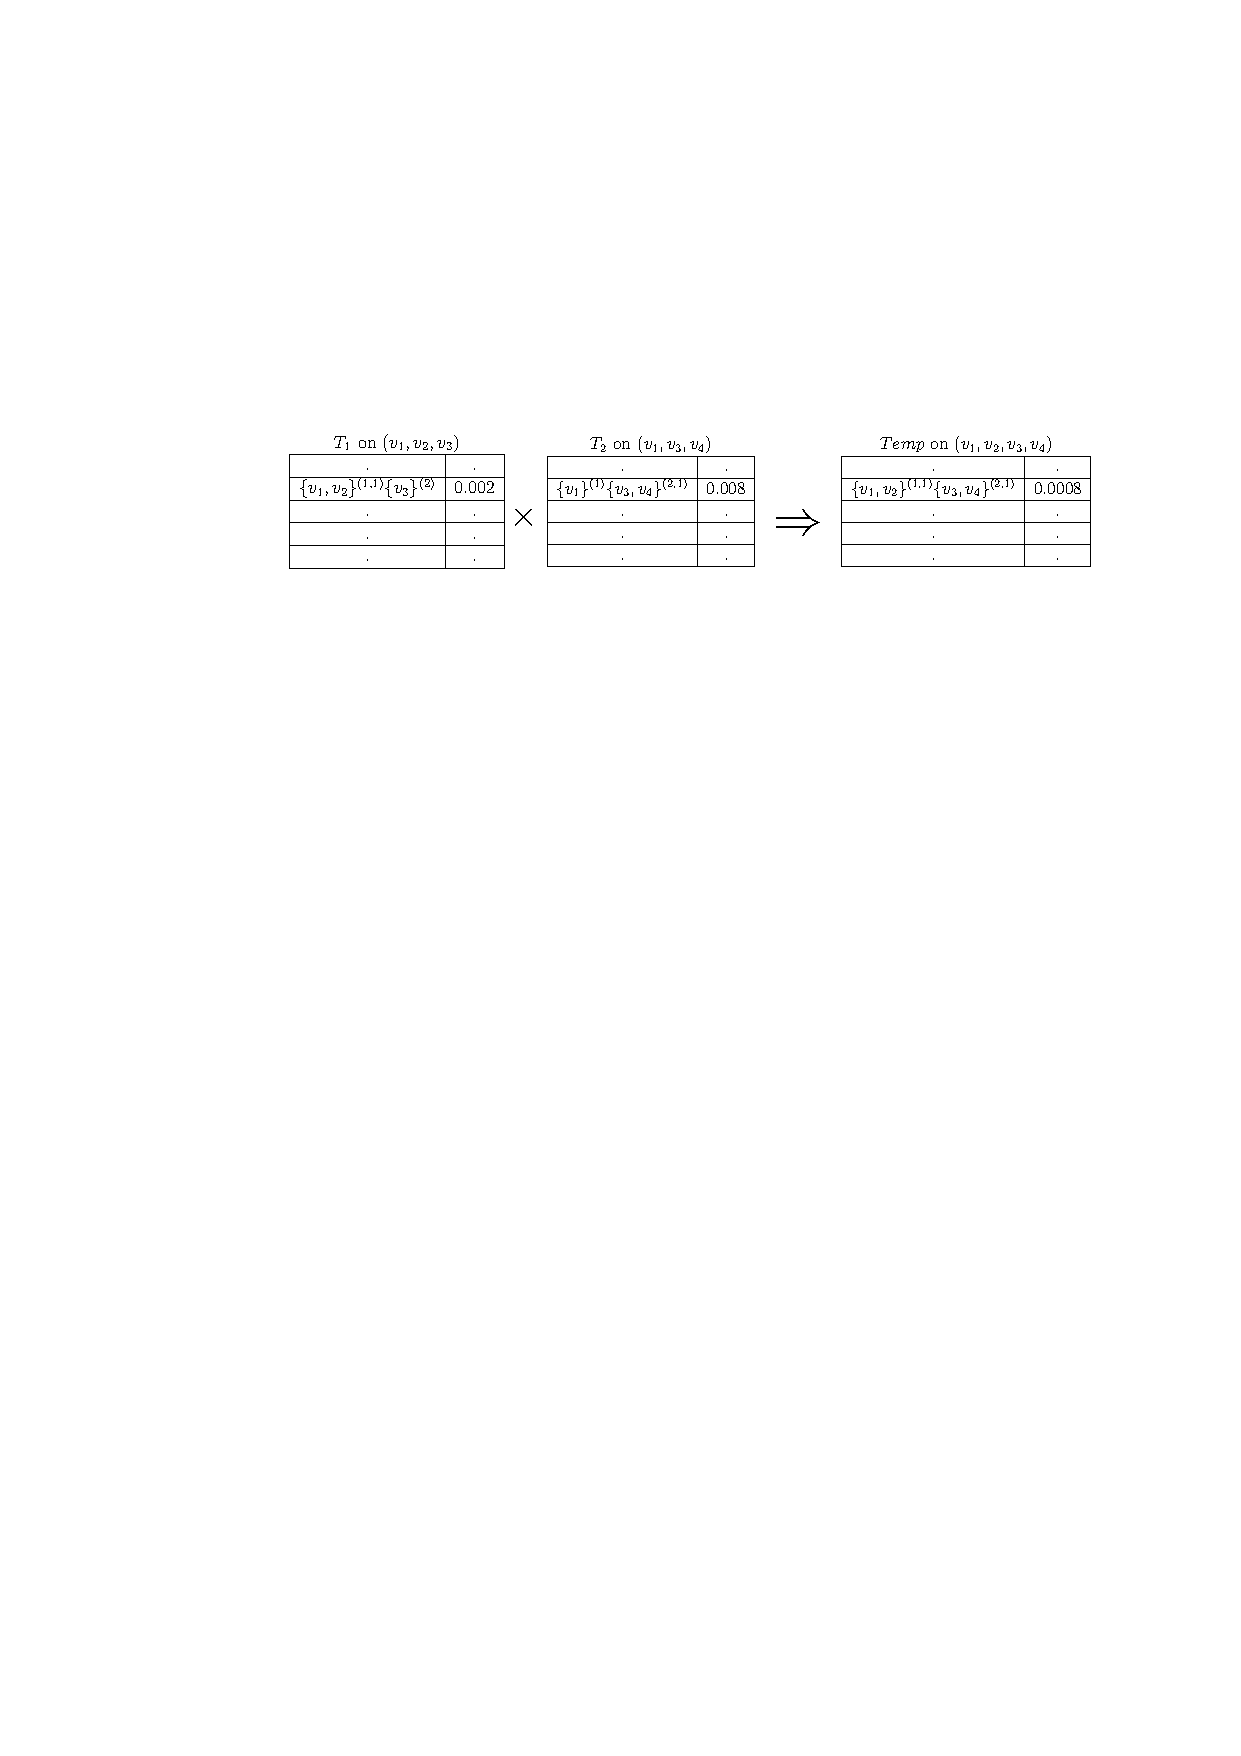
\includegraphics[width=5 in, height=1.2 in]{Table11.pdf}
 \caption{ Merging two tables}.
 \label{fig:table1}
\end{figure}

\begin{example}
\normalfont
Figure \ref{fig:table2} illustrates the operation of the second part of the main loop of function Main in the iteration where node $v_1$ is processed. The table on the left represents $T_{v_i,base}$ after the first part of the main loop finishes. Key $\{v_1,v_2\}^{(1,1)}\{v_3,v_4\}^{(2,1)}$ is good in $T_{v_i,base}$ since $v_1$ is connected to $v_2$ in any network state of this type. Hence, node $v_1$ and its associated position can be deleted from the key. The reduced key appears in the updated $T_{v_i,base}$ on the right.
\end{example}

\begin{figure}[!htb]
\centering
\includegraphics[width=3.5 in, height=1.1 in]{Table111.pdf}
 \caption{ Deleting node $v_i$}.
 \label{fig:table2}
\end{figure}
\section{Correctness}
\label{Sec:crtns}
To prove correctness, we introduce the following notation and definitions.
\begin{enumerate}
\item[{\bf [D1]}]We say that a table $T_{v_i,\alpha}$ is complete with respect to a graph $G_{v_i,\alpha}$ that has been reduced onto the clique $K_{v_i,\alpha}$ if the following conditions hold:
%
\begin{itemize}
%
\item[a)] For each $key\in T_{v_i,\alpha}$, the corresponding value $T_{v_i,\alpha}(key)$ is the probability of obtaining states over the subgraph $G_{v_i,\alpha}$ of type $key$.
%
\item[b)] Each key not in $T_{v_i,\alpha}$ does not contribute to computing the solution $Conn(G)$.
\end{itemize}
%
\end{enumerate}
\nwline
We now show the following theorem.


\begin{theorem} \label{thm:correctnessch4}
\normalfont
At the start of each iteration of the main loop (Step 2) of function Main, if $v_i$ is a node in the current graph then each table $T_{v_i,\alpha}: \alpha=1, 2, \ldots, k, base$, is complete with respect to the graph $G_{v_i,\alpha}$ reduced thus far onto the clique $K_{v_i,\alpha}$.
\end{theorem}
\nwline
\textbf{Proof.}\\
\textbf{Loop Initialization:} At the start of the first iteration, $G$ contains all nodes $V$.
%
In addition, for each clique $K_{v_i,\alpha}$, the subgraph $G_{v_i,\alpha}$ reduced thus far onto the clique $K_{v_i,\alpha}$ is the clique itself (as done in Step 1 of function Main).\\
\nwline
\textbf{Loop Maintenance:} Assume the theorem holds for all possible iterations $r$, where $r\leq n-k-1$. We show that it holds in iteration $r+1$. Let $v_r$ be the $k$-leaf deleted in iteration $r$.
%
Table $T_{v_r,base}$ is the only table that may have changed between iterations $r \mbox{ and } r+1$. 
%
Thus, it suffices to show that $T_{v_r,base}$ is complete with respect to $G_{v_r,base}$. To this end, we note the following in iteration r:

\begin{itemize}
\item Steps 3 to 6 of function Main merge all tables in the set $\{ T_{v_i,\alpha}:\alpha=1, 2, \ldots, k, base \}$ into $T_{v_i,base}$.
\item The loop in Step 7 of function Main discards all bad state types over the graph $\displaystyle \bigcup_{\alpha\in  \{1, 2, \ldots, k, base\}} G_{v_i,\alpha}$. $\blacksquare$
\end{itemize}

%
Following an argument similar to the loop maintenance argument, one can show that at Step 11 in function Main, table $T_{v_{n-k},base}$ associated with the clique $T_{v_{n-k},base}$ containing the sink node is complete with respect to all nodes $V$.
%
Thus, the function returns the required solution.
\section{Running time}
\label{sec:runtym}
Let $n$ be the number of nodes in $G$, $l_{max}$ be the maximum number of locations in the locality set of any node, and $B_k$ be the $k^{th}$ Bell number.
\nwline 
\begin{theorem}\label{thm:runtym}
\normalfont
In the $\ACONN$ algorithm we have
\begin{enumerate}[noitemsep]
\item The maximum length of any table is $\in O(B_k l_{max}^k)$.
\item The worst case running time is $O(n(B_k l_{max}^k)^2)$.
\end{enumerate}
\end{theorem}
\textbf{Proof.}
\nwline
To see (1), we note that the length of each table is determined by the number of partitions of any set of $k$ nodes $(=B_k)$ times the number of different positions that the $k$ nodes can take $(\in O(l_{max}^k))$. Thus, the maximum length of any table is $O(B_k l_{max}^k)$.
\nwline
To see (2), we note that function $t\_merge$ processes $O((B_k l_{max}^k)^2)$ pairs of keys in each call. Function partition merge takes $O(k^3)$ to merge two partitions; this is a constant time for any fixed $k$. Thus, merging two tables requires $O((B_k l_{max}^k)^2)$. 

Function Main processes each node by merging a set of $k\mbox{+}1$ tables. This is done by calling function $t\_merge$ $k$ times. Thus, function Main processes each node in $O(k(B_k l_{max}^k)^2)$. Since $k$ is a constant, processing each node requires $O((B_k l_{max}^k)^2)$. The answer is obtained after processing $n\mbox{-}k$ nodes. Thus, the overall running time is $O(n(B_k l_{max}^k)^2)$. $\blacksquare$
\section{Software Verification}
\label{subsec:vc}
Our devised dynamic programming algorithm is implemented in the $C\mbox{++}$ language with the use of $STL$ (Standard Template Library) container classes.
The program has about 1,300 executable lines (including debugging code). To check the correctness of the implementation, we used the following approaches.
\begin{enumerate}[noitemsep]
\item For probabilistic networks with small number of network states (e.g., $\leq 32$ states) we compare the program output with manual calculations.
\item By definition, if every possible network state is connected then $Conn(G)=1$ regardless of node locations and probability distributions. We verified the output of the program for networks that are manually designed to satisfy this property.

\item Consider two probabilistic networks $G_x$ and $G_y$ where 
\begin{itemize}[noitemsep]
\item $Conn(G_x)=Conn(G_y)=1$, and
\item $x$ and $y$ are distinguished nodes in $G_x$ and $G_y$ respectively.
\end{itemize}
Now, consider the network $G$ obtained from $G_x$ and $G_y$ by introducing a link ($x[i],y[j]$) for some positions of node $x$ and node $y$. No other node in $G_x$ can reach another node in $G_y$. Let $p(x,y)$ be the probability that link $(x,y)$ arises. Then $Conn(G)=p(x,y)$. We utilize the above approach to check correctness.
\item If $G_1, G_2, \mbox{ and } G_3$ are a tree, 2-tree, and 3-tree graphs where $G_1\subset G_2\subset G_3$. Then $Conn(G_1)\leq Conn(G_2)\leq Conn(G_3)$.  Relations of this type are checked in all of the obtained results.
\item For any probabilistic network $G$, using different $PESs$ should result in computing the same $Conn(G)$ value. We used the above property to check our implementation.
\end{enumerate}
\section{Simulation Results}
In this section we present simulation results that explore the following performance aspects of our devised algorithm:
\begin{enumerate}[noitemsep]
\item Execution time of the algorithm
\item Effect of increasing the parameter $k$
\item Effect of increasing node transmission range
\item Effect of $k$-tree subgraph selection method
\end{enumerate}


\begin{figure}[!htb]
\begin{minipage}{.9\linewidth}
\includegraphics[width=6 in, height=2.8 in]{NetworkI_paper.pdf}
\caption{Network $G_{10}$}
\label{fig:netI}
\end{minipage}

\end{figure}
\begin{figure}[!htb]
\begin{minipage}{.9\linewidth}
\includegraphics[width=6 in, height=2.7 in]{NetworkII.pdf}
\caption{Network $G_{12}$}
\label{fig:netII}
\end{minipage}
\end{figure}
\textbf{Test Networks:}
    For simplicity of constructing test networks and analyzing the obtained results, we assume that all nodes have the same transmission range $R_{tr}$, and we set the $E_G$ relation according to the Euclidean distance between the involved nodes.

We have experimented with networks of different sizes in the range $[7,18]$ nodes where each node has a locality set that varies in the range $[2,8]$ rectangles. Here, we  present results on three networks.
\begin{itemize}[noitemsep]
\item Network $G_{10}$ in figure \ref{fig:netI}, consists of $10$ nodes where the locality set of each node varies in the range $[4,6]$.
\item Network $G_{12}$ in figure \ref{fig:netII}, consists of $12$ nodes where the locality set of each node varies in the range $[3,8]$.
\item Network $G_{15}$ in figure \ref{fig:netIII}, consists of $15$ nodes where the locality set of each node varies in the range $[3,6]$.
\end{itemize}
The presented results highlight the most important findings. To avoid cluttering the network diagrams, we omit the $(x, y)$-coordinates of the locality sets. Solid lines in the figures indicate the links used in a spanning tree. Dashed links indicate links of  a 2-tree and dashed dotted links indicate links of a 3-tree.

\begin{figure}[!htb]
\begin{minipage}{.9\linewidth}
\includegraphics[width=6 in, height=2.6 in]{NetworkIII.pdf}
\caption{Network $G_{15}$}
\label{fig:netIII}
\end{minipage}
\end{figure}
   

\begin{enumerate}
\item \textbf{Running Time:} Table \ref{Tab:runtym} shows the obtained running time of the algorithm on each test network when the network is approximated by a tree (solid edges), 2-tree (solid and dashed edges), and 3-tree (all edges). As can be seen, processing 2-trees requires 10 to 15 times more time than processing trees. In addition, processing 3-trees may require 1000 times more time than processing 2-trees.

\begin{table}[!htb]

    %\caption{Global caption}
    %\begin{minipage}{.5\linewidth}
   
      \centering
     \begin{tabular}{|c|c|c|c|}
     \hline
         k& Network $G_{10}$ & Network $G_{12}$ & Network $G_{15}$ \\
     \hline
     1&90& 130& 200 \\\hline
     2&1000 &1380&1480	\\\hline
3 &60000&875000&940000	 \\\hline
\end{tabular}
 \caption{Running time in milliseconds}
\label{Tab:runtym}
\end{table}


\item \textbf{Effect of increasing the parameter $k$:}
Since the set of partial $k$-trees forms a proper subset of partial $k+1$-trees, one may expect that lower bounds obtained by using partial $k$-trees to be generally weaker than lower bounds obtained by using partial $k+1$-trees. This expectation is confirmed by the findings in table \ref{Tab:acc} constructed using networks $G_{10}, G_{12} \mbox{ and } G_{15}$. In the experiments, edges of the used tree, 2-tree, and 3-tree are computed using the greedy method. Table \ref{Tab:acc} indicates that for each of the 3 test networks, we have the following relation $\frac{Conn(\mbox{2-tree})}{Conn(\mbox{tree})}>\frac{Conn(\mbox{3-tree})}{Conn(\mbox{2-tree})}$.
 %\begin{minipage}{.5\linewidth}

   \begin{table}[!htb] 
      \centering
     \begin{tabular}{|c|c|c|c|}
     \hline
      k& Network $G_{10}$ & Network $G_{12}$ & Network $G_{15}$ \\
     \hline
      1 & 0.62&0.336& 0.82 \\\hline
2 &0.71 & 0.36& 0.99\\\hline
3 &0.75& 0.37& 1\\\hline
\end{tabular}
 \caption{Connectivity lower bounds using different partial $k$-trees}
 \label{Tab:acc}
\end{table}

\item \textbf{Effect of increasing node transmission range:} Intuitively, increasing node transmission range $R_{tr}$ of a given probabilistic network $G$ has two effects:
\begin{enumerate}
\item increasing the number of edges in the network and
\item increasing the probability that any given edge arises.
\end{enumerate}
 Consequently, denser partial $k$-tree subgraphs with better edge probabilities can be found. Thus, $Conn(G)$ is expected to increase. Figure \ref{fig:res} explores this aspect for network $G_{10}$ when $R_{tr}$ varies in the range $[5.5, 9.5]$ and a tree (partial 2-tree, or 3-tree) subgraph is selected randomly. As can be seen, bounds obtained by using a tree (2-tree, or a 3-tree) increases as $R_{tr}$ increases.

\begin{figure}[!htb]
\begin{minipage}[]{.5\linewidth}
\includegraphics[width=3 in, height=2.5 in]{random1.pdf}
 \caption{ Connectivity versus transmission range with random subgraph selection}
\label{fig:res}
\end{minipage}
\begin{minipage}{.5\linewidth}
\includegraphics[width=3 in, height=2.5 in]{selective1.pdf}
 \caption{ Connectivity versus transmission range with greedy subgraph selection}
\label{fig:ges}
 \end{minipage}
\end{figure}

%\begin{figure}[!htb]
%\begin{minipage}[]{1\linewidth}
%\includegraphics[width=6 in, height=2.5 in]{output.pdf}
% \caption{ Connectivity versus transmission range with  random edge selection.
%}
%\label{fig:res}
%\end{minipage}
%\end{figure}
\item {\bf Effect of subgraph selection method:} Intuitively, for any given $k$, lower bounds obtained from partial $k$-tree subgraphs obtained using the greedy method (c.f. Chapter 2) are likely to be better than lower bounds obtained using the random method. To investigate this aspect, we compute lower bounds on network $G_{10}$ (used to generate figure \ref{fig:ges}) when we use partial $k$-tree subgraphs computed using the greedy method. The obtained results confirm the above intuition. For example, consider the bounds obtained by using tree subgraphs when $R_{tr}=6$. For this scenario, figure \ref{fig:res} gives  $Conn(G)\geq 0$ whereas figure \ref{fig:ges} gives $Conn(G)\geq 0.1$
\end{enumerate}



\section{Concluding Remarks}
In this chapter, we have extended the dynamic programming approach used in Chapter 3 to handle the $\ACONN$ problem on any probabilistic network whose underlying graph is a partial $k$-tree $G$, assuming that a $PES$ of $G$ is given. The algorithm runs in polynomial time for any fixed $k$. It provides a network design tool for analyzing probabilistic connectivity when any combination of the following parameters change: node locality sets, their probabilistic distribution, and node transmission range.     
\chapter{Networks with Relays}
\begin{quote}
In this chapter, we extend the dynamic program of Chapter 4 for solving the $\ACONN$ problem on partial $k$-trees to solve the $\ARCONN$ and $\SRCONN$ problems. For each problem, we present the modifications required, analyze the running time, and present simulation results to explore some performance and usage aspects.
\end{quote}


\section{Overview of the Extensions}
\label{sec:overviewExt}
Throughout this chapter, the UWSN is modelled by a probabilistic graph $G=(V=V_{sense}\cup V_{relay}$ $,E_G,Loc,p)$ where $V=V_{sense}\cup V_{relay}$, and $V_{relay}$ may contain zero or more relay nodes. As in Chapter 4, we assume that $G$ has the topology of a partial $k$-tree for some specified $k$. In addition, when no confusion arises, we use $G$ to refer also to the partial $k$-tree graph underlying the structure of the probabilistic graph $G$.

%
Our proposed extended algorithm for solving the $\ARCONN$ and  $\SRCONN$ problems have the same structure and organization as the algorithm presented in Chapter 4.
%
Functions Main and $t\_merge$ (but not $p\_merge$) are modified, but maintain their high level structure and steps.
As discussed below, the main modifications concern the formulation of new network state types to solve each problem. The modifications introduce new steps to initialize and maintain the new state types, as well as extract a final solution from them.

\section{The $\ARCONN$ Algorithm}
\label{sec:arconnalg}
We present below the needed modifications to solve the $\ARCONN$ problem.
\subsection{$\ARCONN$ State Types}
\begin{definition}[\textbf{state types of the $\ARCONN$ problem}]\label{def:arconnstatety}
\normalfont
Let $G_{v_i,\alpha}$ be a subgraph reduced onto clique $K_{v_i,\alpha}$. Denote by $V_{v_i,\alpha}$ the set of nodes of the graph $G_{v_i,\alpha}$. Let $S=\{v_a[i_a] :v_a\in V_{v_i,\alpha} \mbox{ and } i_a \in Loc(v_a)\}$  be a network state of $G_{v_i,\alpha}$. \\Then\\
\centerline{
$AR\mbox{-}type(S)=\{V_{1,b(V_1)}^{Loc(V_1)}, V_{2,b(V_2)}^{Loc(V_2)}, \ldots, V^{Loc(V_r)}_{r,b(V_r)} \}$}

where
\begin{itemize}[noitemsep]
\item $\{V_1^{Loc(V_1)}, V_2^{Loc(V_2)}, \ldots, V_r^{Loc(V_r)}\}=A\mbox{-}type(S)$
\item For each part $V_i\subseteq V_{v_i,\alpha}$ of the partition $(V_1,V_2,\ldots,V_r)$, $b(V_i)$ is a binary $(0/1)$ indicator. To explain the setting of $b(V_i)$, let us denote by $S_i \subseteq S$ the connected component of state $S$ that contains all nodes in $V_i$. We set $b(V_i)=1$ if $S_i$ contains at least one sensor node from $V_{sense}$. Else (if $S_i$ is composed of relay nodes only), then $b(V_i)=0$.
 $\blacksquare$
\end{itemize}
\end{definition}

\begin{example}
\normalfont
In figure \ref{fig:sttype1}, denote by $G_{v_i,1}$, the graph induced on nodes $\{v_a,v_b,v_i,v_j,v_k\}$. Assume that $\{v_b\}\in V_{sense}$ and $\{v_a,v_i,v_j,v_k\} \in V_{relay}$. Suppose that state $S$ of figure \ref{fig:sttype1_node} is a possible network state of $G_{v_i,1}$. Then $AR\mbox{-}type(S)=\big \{\{v_i\}_1^{(1)},\{v_j,v_k\}_0^{(2,3)}\big\}$. Here, the indicator $b(\{v_i\})=1$ since $v_b$ is a sensor node connected to $v_i$ in $S$. $\blacksquare$
\end{example}
\begin{figure}[!htb]
\begin{minipage}[]{0.5\linewidth}
\includegraphics[width=2.2 in, height=1.8 in]{Ch5f2.pdf}
\caption{A fragment of a 3-tree}
\label{fig:sttype1}
\end{minipage}
\begin{minipage}{0.5\linewidth}
\nwline
\includegraphics[width=1.7 in, height=1.5 in]{Ch5f2_1.pdf}
\caption{A state $S$ on $\{v_a,v_b,v_i,v_j,v_k\}$}
\label{fig:sttype1_node}
\end{minipage}
\end{figure}
The rationale behind the definition of $AR\mbox{-}types$ is that when we merge tables containing information of two subgraphs $G_{v_i,1}$ and $G_{v_i,2}$ to compute summary information of the union graph $G_{v_i,1}\cup G_{v_i,2}$, we need to know which connected components contain at least one sensor node (and thus, are essential to form an operating state), or contain relay nodes only (and thus, may not be essential to form an operating state). 
\subsection{Initializing Tables}
\label{subsec:initt}
Step 1 of function Main initializes a table $T_H$ associates with each $k$-cliques $H$ of the full graph $k$-tree($\tilde{G}$).
Similar to the approach used in Chapter 4, we perform the following steps,
\begin{enumerate}[noitemsep]

\item We construct for each edge $e=\{x,y\}$ in $H$ an exhaustive table $T_e$ where the keys are of the $AR$-$type$.
\item We use $t\_merge$ and $p\_merge$ to compute the cross product of all tables associated with all edges in the $k$-clique $H$.
\end{enumerate}

\subsection{Merging $\ARCONN$ State Types}
\label{subsec:mst}

We recall that function $t\_merge$ takes as input two table $T_1$ and $T_2$ that may have a set $C=V(T_1)\cap V(T_2)$ of common nodes, and produces a new table $T_{out}$. The context of the merge operation is as follows. 


Each table $T_i, i=1,2,$ contains summary information about a subgraph $G_i$ that has been reduced onto a clique $K_i$. The merge operation computes a table $T_{out}$  that stores summary information about the graph $G_1\cup G_2$.

$T_{out}$ is computed by processing each pair of keys (i.e., $\ARCONN$ state types) $key_1\in T_1$ and $key_2\in T_2$. Processing $key_1 \mbox{ and } key_2$ results in a new state type, denoted $key_{out}$, and an associated probability, denoted $p_{out}$.
%
To explain processing of $key_1$ and $key_2$, consider two network states: $S_i, i=1,2,$ of the subgraph $G_i$ reduced onto the clique $K_i$, where $key_i=AR\mbox{-}type(S_i)$. Merging $S_1$ and $S_2$ generates $key_{out}=AR\mbox{-}type(S_1\cup S_2)$.

As in Chapter 4, such a union is possible only if each common node in $C$ assumes the same position in both of $S_1$ and $S_2$. Else, the two keys are not compatible, and no $key_{out}$ is generated.

To explain the structure of $key_{out}$ (if it exists), let\\
\nwline
\begin{center}
$\begin{array}[t]{l}
AR\mbox{-}type(S_1)=\{X_{i,b(X_i)}^{Loc(X_i)} : i=1,2, \ldots\},\\
AR\mbox{-}type(S_2)=\{Y_{j,b(Y_j)}^{Loc(L_j)} : j=1,2, \ldots\}, and\\
AR\mbox{-}type(S_1\cup S_2)=\{Z_{k,b(Z_k)}^{Loc(Z_k)} : k=1,2, \ldots\}\end{array}$.
\end{center}
Then 
\begin{itemize}[noitemsep]
\item The partition $\{Z_k:k=1,2,\}$ is generated by applying partition merge to $\{X_i:i=1,2,\ldots\}$ and $\{Y_j:j=1,2,\ldots\}$.
\item The binary indicator obtained by merging two parts, say $X_i$ and $Y_j$ is  $max(b(X_i),b(Y_j))$.
\end{itemize}
Similar to the $\ACONN$ algorithm, the probability $p_{out}$ is the product $T_1(key_1) \times T_2(key_2)$ divided by a correction term  $=\prod \big (p_x(i):x[i] \mbox{ is common between } key_1 \mbox{ and } key_2\big)$.

%%%%
%Example 5.6 Same as example 4.6
%

\subsection{Removing Bad State Types}
\label{subsec:rbst}
We recall that the first part of the main loop of function Main merges all tables $\{T_{v_i,\alpha} :\alpha=base,1,2, \ldots,k\}$ into table $T_{v_i,base}$. The second part of the main loop (Steps 7 to 10) removes bad state types from table $T_{v_i,base}$ prior to deleting node $v_i$.
%
For the $\ARCONN$ problem, a state $S$ of the subgraph $G_{v_i,base}$ reduced onto the $k$-clique $K_{v_i,base}$ is considered bad at this stage if node $v_i$ appears as a singleton part in the partition associated with $AR\mbox{-}type(S)$ and the indicator $b({v_i})=1$.


 This badness follows since $S$ has a connected component with at least one sensor node, and this component reaches outside nodes via node $v_i$, yet node $v_i$ is disconnected from other nodes in $K_{v_i,base}$. The algorithm removes all such bad state types from $T_{v_i,base}$.

Else if $AR\mbox{-}types(S)$ is good then one of the following cases applies:
\begin{itemize}[noitemsep]
\item \textbf{Case: $v_i$ is a singleton part and $b(\{v_i\})=0$}. Here, the part $\{v_i\}$ is merely removed from $AR\mbox{-}type(S)$.
\item \textbf{Case: $v_i$ is not singleton}. Assume that $v_i$ belong to part $V_1$, where $|V_1|\geq 2$. Then node $v_i$ and its associated position is removed from $V_1$.
\end{itemize}

\subsection{Obtaining Final Result}
\label{subsec:ofr}
Step 11 of function Main is modified to compute $Conn(G)$ as the sum of all values in table $T_{v_{n-k},base}$ corresponding to $AR\mbox{-}types$ of the form\\
\nwline
\centerline{
$\{X_{i,b(X_i)}^{Loc(X_i)} : i=1,2, \ldots\}$}
where
\begin{itemize}[noitemsep]
\item the particular part of the partition ${X_1,X_2,\ldots,X_r}$ that contains the sink node, say $X_1$, has $b(X_1)=1$, and 
\item each other part $X_j, j \neq 1,$ of the partition has $b(X_j)=0$.
\end{itemize}
That is, step 11 considers only network states where any connected component disconnected from the sink does not have any sensor node. Thus, all sensor nodes must lie in the same component of the sink node.

\subsection{Running Time}
\label{subsec:rt}

As in Chapter 4, $n$ denotes the number of nodes in $G$, $l_{max}$ denotes the maximum number of locations in the locality set of any node, and $B_k$ denote the $k^{th}$ Bell number.
\begin{theorem}\normalfont In the $\ARCONN$ algorithm we have\label{thm:rt}
\begin{enumerate}[noitemsep]
\item The maximum length of any table is $O(B_kl_{max}^k2^k)$ 
\item The worst case running time is $O(n(B_kl_{max}^k2^k)^2)$
\end{enumerate}
\end{theorem}


The proof is similar to the proof of the Theorem \ref{thm:runtym} by observing that adding indicator bits to state types makes the maximum table length as specified in part 1.
\section{$\ARCONN$ Simulation Results}
\label{sec:arconnsim}
Relay nodes are expected to be cheaper than sensor nodes since they do not include sensing devices. In addition, relay nodes are not required to do energy consuming data acquisition tasks as sensor nodes. Hence, their design may enjoy more flexibility than sensor nodes, and their energy supply is expected to last longer.

In this section we utilize the algorithm developed for the $\ARCONN$ problem to investigate the positive effects of deploying relay nodes.
\begin{figure}[!htb]
\begin{minipage}{.9\linewidth}
\includegraphics[width=6 in, height=2.8 in]{NetworkI_paper.pdf}
\caption{Network $G_{10}$}
\label{fig:netI1}
\end{minipage}
\end{figure}

\begin{figure}[!htb]
\begin{minipage}{.9\linewidth}
\includegraphics[width=6 in, height=2.8 in]{NetworkI_paper_Relay.pdf}
\caption{Network $G_{10,3}$}
\label{fig:netIR}
\end{minipage}
\end{figure}

\textbf{Test Networks:} To illustrate our basic findings, we present results on network $G_{10}$ (figure \ref{fig:netI1}) and network $G_{10,3}$ (figure \ref{fig:netIR}) which adds 3 relay nodes to $G_{10}$. In each network, $v_1$ is the sink node, and all edges shown in the figures appear when $R_{tr}\geq 6.5$ units. Reducing $R_{tr}$ results in networks with possibly fewer edges. We experiment with a tree, 2-tree, and 3-tree subgraphs shown by the solid and dotted lines in the figure. The subgraphs are obtained using the greedy method of Chapter 2.

\begin{enumerate}
\item \textbf{Running Time:} Table \ref{Tab:rtym1} shows the increase of running time as the dynamic program moves from using $A\mbox{-}type$ keys on $G_{10}$ to using $AR\mbox{-}type$ keys on $G_{10,3}$ 
\begin{table}[!htb]
    %\caption{Global caption}
    \begin{minipage}{1\linewidth}
   
      \centering
     \begin{tabular}{|c|c|c|}
     \hline
         k& Network $G_{10}$ &Network $G_{10,3}$\\
     \hline
     1&90& 110 \\\hline
     2&1000 &6000	\\\hline
3 &6000&8000	 \\\hline
\end{tabular}
 \caption{Running time in milliseconds}
\label{Tab:rtym1}
    \end{minipage}
\end{table}
\item \textbf{Effect of adding relay nodes:} Table \ref{Tab:SRC} shows the obtained bounds on $G_{10}$ and $G_{10,3}$. As can be seen, adding 3 relay nodes can enhance the computed $Conn(G)$ by, e.g. $63\%$ (the $3^{rd}$ row).


\begin{table}[!htb]
  \centering
 \begin{minipage}{.5\linewidth}
     \begin{tabular}{|c|c|c|}
     \hline
     k & Network $G_{10}$ & Network $G_{10,3}$  \\
     \hline
      1 & 0.30 & 0.86 \\\hline
	  2 & 0.54 & 0.96\\\hline
	  3 &0.60 & 0.98 \\\hline
\end{tabular}
    \end{minipage}
     \caption{Connectivity with respect to $k$}
      \label{Tab:SRC}   
\end{table}
\item \textbf{Effect of adding relay nodes for various node $R_{tr}$:}
Figure \ref{Fig:NWOR} illustrates $Conn(G)$, on  $G_{10}$ and $G_{10,3}$ as $R_{tr}$ varies in the range $[2.5,7.5]$. Each obtained curve exhibits a notable monotonic increasing behaviour as $R_{tr}$ increases. As explained in Chapter 4, this behaviour is due to the appearance of more edges as $R_{tr}$ increases, and the potential increase in the probability of each edge as $R_{tr}$ increases. Increasing $R_{tr}$, however, requires increasing node energy consumption. To achieve a desired $Conn(G)$ value, a designer may utilize the obtained curves to assess the merit of increasing $R_{tr}$ versus deploying more relay nodes.
\begin{figure}[!htb]
\begin{minipage}{.9\linewidth}
\end{minipage}
\includegraphics[width=6 in, height=2.6 in]{NetworkI_woR.eps}
\caption{Connectivity versus transmission range}
\label{Fig:NWOR}
\end{figure}

\end{enumerate}






\section{The $\SRCONN$ Algorithm}
\label{sec:sralg}
Next, we present the needed modifications to solve the $\SRCONN$ problem.
\subsection{$\SRCONN$ State Types}
\label{subsec:srst}

\begin{definition}[\textbf{state types of the $\SRCONN$ problem}]\label{def:srst}
Let $G_{v_i,\alpha}$ be a subgraph reduced onto a clique $K_{v_i,\alpha}$. Denote by $V_{v_i,\alpha}$ the set of nodes of the graph $G_{v_i,\alpha}$. Let $S=\{v_a[i_a] :v_a\in V_{v_i,\alpha} \mbox{ and } i_a \in Loc(v_a)\}$  be a network state of $G_{v_i,\alpha}$.\\
Then
\nwline
\centerline{
$SR\mbox{-}type(S)=\{V_{1,c(V_1)}^{Loc(V_1)}, V_{2,c(V_2}^{Loc(V_2)}, \ldots, V^{Loc(V_r)}_{r,c(V_r} \}$}

where
\begin{itemize}[noitemsep]
\item $\{V_1^{Loc(V_1)}, V_2^{Loc(V_2)}, \ldots, V_r^{Loc(V_r)}\}=A\mbox{-}type(S)$
\item For each part $V_i\subseteq V_{v_i,\alpha}$ of partition $(V_1,V_2,\ldots,V_r)$, $c(V_i)$ is the number of sensor nodes in the connected component $S_i \subseteq S$  that includes all nodes in $V_i$.
 $\blacksquare$
\end{itemize}
\end{definition}

\begin{example}
\normalfont
 In figure \ref{fig:sttype2}, denote by  $G_{v_i,1}$, the graph induced on nodes $\{v_a,v_b,v_i,v_j,v_k\}$. Assume that $\{v_b,v_i\}\in V_{sense}$ and $\{v_a,v_j,v_k\} \in V_{relay}$. Suppose that state $S$ of figure \ref{fig:sttype2_node} is a possible network state of $G_{v_i,1}$. Then $SR\mbox{-}type(S)=\big \{\{v_i\}_2^{(1)},\{v_j,v_k\}_0^{(2,3)}\big\}$. Here, the count $c(\{v_i\})=2$ since both of $v_i$ and $v_b$ are sensor nodes.
 $\blacksquare$
\end{example}
\begin{figure}[!htb]
\begin{minipage}[]{0.5\linewidth}
\includegraphics[width=2.2 in, height=1.8 in]{Ch5f3.pdf}
\caption{A 3-tree fragment}
\label{fig:sttype2}
\end{minipage}
\begin{minipage}{0.5\linewidth}
\includegraphics[width=1.7 in, height=1.5 in]{Ch5f3_1.pdf}
\caption{A state $S$ on $\{v_a,v_b,v_i,v_j,v_k\}$}
\label{fig:sttype2_node}
\end{minipage}
\end{figure}
The rationale behind the definition of the $SR\mbox{-}type$ is that when we merge tables containing summary information of two subgraphs $G_1$ and $G_2$ to compute summary information of the union graph $G_1\cup G_2$, we need to know  how many sensor nodes are in each connected component of each state $S$ summarized in the class $SR\mbox{-}type(S)$.


\subsection{Initializing Tables}

Step 1 of function Main initializes a table $T_H$ associates with each $k$-cliques $H$ of the full graph $k$-tree($G$). Our approach here is similar to the one used in Section \ref{subsec:initt}

\subsection{Merging $\SRCONN$ State Types}
\label{subsec:msst}
Using the same notation of section \ref{subsec:mst}, we explain how to process a pair of keys: $key_1\in T_1$ and $key_2\in T_2$, where $T_1$ and $T_2$ are two tables to be merged.

We consider two network states: $S_i, i=1,2,$ where $S_i$ is a network state of the subgraph $G_i$ reduced onto the clique $K_i$, where $key_i=SR\mbox{-}type(S_i)$. Merging $S_1$ and $S_2$ generates $key_{out}=SR\mbox{-}type(S_1\cup S_2)$.

As  with keys of the $A\mbox{-}type$ (or $AR\mbox{-}type$) the union $S_1 \cup S_2$ is possible only if each common node between $S_1$ and $S_2$ takes the same position in both states.

Now, let
\begin{center}
$\begin{array}[t]{l}
SR\mbox{-}type(S_1)=\{X_{i,c(X_i)}^{Loc(X_i)} : i=1,2, \ldots\},\\

SR\mbox{-}type(S_2)=\{Y_{j,c(Y_j)}^{Loc(L_j)} : j=1,2, \ldots\}, \mbox{and}\\
SR\mbox{-}type(S_1\cup S_2)=\{Z_{k,c(Z_k)}^{Loc(Z_k)} : k=1,2, \ldots\}\end{array}$\\
\end{center}

Then 
\begin{itemize}[noitemsep]
\item The partition $\{Z_k:k=1,2,\}$ is generated by applying partition merge to $\{X_i:i=1,2,\ldots\}$ and $\{Y_j:j=1,2,\ldots\}$.
\item If parts $X_i$ and $Y_j$ are merged together into $Z_k$, and the number of common sensor nodes between $X_i$ and $Y_j$ is denoted $n_{ij}$ then\\
\nwline
\centerline{
$c(Z_k)=max(n_{req},c(X_i)+c(Y_j)-n_{ij})$.
	}
\end{itemize}
Similar to the $\ACONN$ algorithm, the probability $p_{out}$ is the product $T_1(key_1) \times T_2(key_2)$ divided by a correction term  $=\prod (p_x(i):x[i] \mbox{ is common between } key_1 \mbox{ and } key_2)$.

\subsection{Bad State Types}
\label{subsec:bst}

Using the same context and notation of section \ref{subsec:rbst}, we define in this section bad $\SRCONN$ state types. For a given node $v_i$ that is processed  in some iteration of the main loop of function Main, the first part of function Main merges all tables $\{T_{v_i,\alpha} :\alpha=1,2, \ldots,k,base\}$ into table $T_{v_i,base}$.

For a state $S$ of $G_{v_i,base}$, let $n_{sense}(S)$ be the number of sensor nodes that can reach the rest of the graph by nodes in the separator clique $K_{v_i,base}$.
Thus, if $SR\mbox{-}type(S)=\{X_{i,c(X_i)}^{Loc(X_i)}: i=1,2, \ldots,r\}$  then
\nwline
\[
 n_{sense}(S) =
  \begin{cases}
   \displaystyle\sum_{X_j\neq\{v_i\}} c(X_j)  & 
   \begin{array}[t]{l}
   \mbox{if node } v_i \mbox{ appears as a singleton in the partition}\\ (X_1,X_2,\ldots,X_r)
    \end{array}\\
   \displaystyle\sum_{j=1,2,\ldots,r}  c(X_j)   & \mbox{ otherwise}
  \end{cases}
\]
\nwline
Now, let us denote by $n_{v_i,base,sense}$ the number of sensor nodes in the  subgraph $G_{v_i,base}$ reduced onto the $k$-clique $K_{v_i,base}$ at the end of the first part of the main loop in function Main. Thus, $|V_{sense}|-n_{v_,base,sense}$ is the number of sensor nodes outside the graph $G_{v_i,base}$.
By definition of operating states of the $\SRCONN$ problem, $SR\mbox{-}type(S)$ is bad if 

\centerline{$n_{sense}(S)+(|V_{sense}|-n_{v_i,base,sense})\leq n_{req}$.}


We recall that the algorithm removes all such bad state types from $T_{v_i,base}$ in step 9 of function Main. Else, if $SR\mbox{-}type(S)$ is good then the algorithm just removes node $v_i$ and its associated position from $SR\mbox{-}type(S)$.

\subsection{Obtaining Final Result}
\label{subsec:ofr1}
Step 11 of function Main computes $Conn(G,n_{req})$ as the sum of all values in the table $T_{v_{n-k},base}$ corresponding to keys of the form \\
\nwline
\centerline{
$\{X_{i,c(X_i)}^{Loc(X_i)} : i=1,2, \ldots\}$}
\nwline
where the partition part that contains the sink node, say $X_1$, has $c(X_1)\geq n_{req}$.

\subsection{Running Time}
\label{subsec:rt1}
As in Chapter 4, $n$ denotes the number of nodes in $G$, $l_{max}$ denotes the maximum number of locations in the locality set of any node, and $B_k$ denote the $k^{th}$ Bell number.
\begin{theorem}\normalfont In the $\SRCONN$ algorithm we have\label{thm:rt1}
\begin{enumerate}
\item The maximum length of any table is $O(B_kl_{max}^kn_{req}^k)$ 
\item The worst case running time is $O(n(B_kl_{max}^kn_{req}^k)^2)$
\end{enumerate}
\end{theorem}

The proof is similar to the proof of the Theorem \ref{thm:runtym} by observing that adding the counters $c(V_i)$ to state types makes the maximum table length as specified in part 1.

\section{$\SRCONN$ Simulation Results}
\label{sec:srconnsim}
The $\SRCONN$ problem is motivated by applications where an UWSN task can be achieved by any subset of sensor nodes connected the sink and has $\textrm{size}\geq n_{req}$ nodes, where $n_{req}$ is a design parameter.
For such applications, a designer has at least 3 options to achieve a minimum required $Conn(G,n_{req})$ value:

\begin{itemize}
\item tuning the $n_{req}$ parameter,
\item tuning node transmission range $R_{tr}$, and
\item tuning the number of deployed relay nodes.
\end{itemize}
In this section we explore the use of our devised $\SRCONN$ algorithm to tackle such design problem.


\textbf{Test Networks:} As in section \ref{sec:arconnsim}, we use network $G_{10}$ in figure \ref{fig:netI1} and $G_{10,3}$ in figure \ref{fig:netIR}


\textbf{Effect of varying $n_{req}$:} Figure \ref{Fig:CvCwr1} illustrates the achieved $Conn(G,n_{req})$ as $n_{req}$ varies in the range $[1,10]$. Figure \ref{Fig:CvCwr2} illustrates the achieved $Conn(G,n_{req})$ as $n_{req}$ varies in the range $[1,10]$, and $R_{tr}$ varies in the range $[2.5,5.5]$.

\begin{figure}[!htb]
\begin{minipage}{0.5\linewidth}
\centering
\includegraphics[width=3 in, height=2.4 in]{abc.pdf}
\caption{Connectivity versus $n_{req}$}
\label{Fig:CvCwr1}
\end{minipage}
\begin{minipage}{0.5\linewidth}
\centering
\includegraphics[width=3 in, height=2.4 in]{3D.pdf}
\caption{Connectivity versus $n_{req}$ and transmission range}
\label{Fig:CvCwr2}
\end{minipage}
\end{figure}

\section{Concluding Remarks}
In this chapter we have presented extensions to the $\ACONN$ dynamic programming algorithm. The extensions yield two algorithms for solving the $\ARCONN$ and $\SRCONN$ problem on partial $k$-trees where a $k$-$PES$ is specified for each problem instance. The algorithms run in polynomial time on any partial $k$-tree with fixed $k$. The algorithms are implemented in $C\mbox{++}$ and provide network design tools for analyzing probabilistic connectivity when any combination of the following parameters change: node locality sets and their probabilistic distribution, node transmission range, number of relay nodes that can be deployed, and the number of nodes connected to the sink required achieve a given task.  
 
\chapter{Concluding Remarks}
% Need to writedown our contribution
The work in this thesis has been motivated by recent interest in UWSNs as a platform for preforming many useful tasks. A challenge arises since sensor nodes incur small scale and large scale movements that can disrupt network connectivity. Thus, tools for quantifying the likelihood that a network remains completely or partially connected become of interest.

To this end, the thesis has formalized 4 probabilistic connectivity problems, denoted $\ACONN,$ $ \SCONN, \ARCONN, \mbox{ and } \SRCONN$. The obtained results show that all of the 4 problems admit polynomial time algorithms on $k$-trees (and their subgraphs), for any fixed $k$. The running times of the algorithms, however, increase exponentially as $k$ increases. Thus, more work needs to be done towards obtaining more effective algorithms.\\
For future research, we propose the following directions.
\begin{itemize}[noitemsep]
\item As mentioned in Chapter 1, the class of probabilistic connectivity problems discussed in the thesis shares some similarity with the class of network reliability problems discussed in \cite{Co87, shier1991network}. Both classes of problems utilize a type of probabilistic graphs to formalize the problems, and core problems in each class are $\#P\mbox{-}hard$ problems.

In ~\cite{Co87}, a number of methods are devised to cope with the problems. These methods aim at finding classes of graphs for which the problems can be solved effectively, as well as deriving lower and upper bounds from disjoint or overlapping subgraphs that form either pathsets or cutsets. Investigating the applicability of such methods to probabilistic connectivity problems appears to be a worthwhile direction.

\item Some wireless sensor network applications require that sensor nodes repeatedly perform data collection rounds. In each round, sensor nodes collect data and forward the collected data to the sink node using multihop routes. Existing results in the literature (e.g., \cite{pu2013comparing}) have shown that the direction of water currents influence delays in underwater acoustic communication. Given randomness in the position of UWSN nodes, it becomes interesting to analyze the delays incurred in typical data collection rounds.
\item Area coverage analysis is a topic that has received attention in UWSNs. In light of node mobility in UWSNs, it appears worthwhile to investigate area coverage assuming a probabilistic locality model of the nodes.
\end{itemize}


 
%
%%----------------------------------------------------------------------------------------
%%	THESIS CONTENT - APPENDICES
%%----------------------------------------------------------------------------------------
%
%\addtocontents{toc}{\vspace{2em}} % Add a gap in the Contents, for aesthetics
%
%\appendix % Cue to tell LaTeX that the following 'chapters' are Appendices
%
%% Include the appendices of the thesis as separate files from the Appendices folder
%% Uncomment the lines as you write the Appendices
%
%\input{Appendices/AppendixA}
%%\input{Appendices/AppendixB}
%%\input{Appendices/AppendixC}
%
%\addtocontents{toc}{\vspace{2em}} % Add a gap in the Contents, for aesthetics
%
%\backmatter

%----------------------------------------------------------------------------------------
%	BIBLIOGRAPHY
%----------------------------------------------------------------------------------------

\label{Bibliography}

\lhead{\emph{Bibliography}} % Change the page header to say "Bibliography"

\bibliographystyle{plain} % Use the "unsrtnat" BibTeX style for formatting the Bibliography

\bibliography{Bibliography} % The references (bibliography) information are stored in the file named "Bibliography.bib"

\end{document}  